\documentclass[11pt,a4paper]{article}
\usepackage[margin=2.2cm]{geometry}
\usepackage[T1]{fontenc}
\usepackage{lmodern,microtype}
\usepackage{amsmath,amssymb,bm}
\usepackage{graphicx,booktabs,siunitx,multirow,array,tabularx}
\usepackage{xcolor}
\usepackage{tikz}
\usetikzlibrary{positioning,arrows.meta,fit,backgrounds,calc}
\usepackage[hidelinks]{hyperref}
\usepackage[nameinlink,capitalise]{cleveref}
\usepackage{enumitem}
\usepackage{adjustbox}
\usepackage{caption}
\setlist{nosep,leftmargin=*}
\sisetup{detect-all}
\setlength{\emergencystretch}{3em}
\graphicspath{{../docs/figures/}}
\newcommand{\R}{\mathbb{R}}
\newcommand{\vect}[1]{\bm{#1}}
\newcommand{\ok}{\textcolor{green!50!black}{\textbf{pass}}}
\newcommand{\pend}{\textcolor{orange!80!black}{\textbf{partial}}}
\newcommand{\no}{\textcolor{red!70!black}{\textbf{not done}}}

\title{\textbf{quadsim}: A Modular, Validated Drone Reinforcement-Learning Research Framework on NVIDIA Isaac Lab\\[4pt]
\large Technical Report}
\author{Drone\_Sim\_RL project}
\date{November 2026}

\begin{document}
\maketitle

\begin{abstract}
We present \emph{quadsim}, a GPU-parallel quadrotor simulation and reinforcement-learning (RL) platform built on
Isaac Lab~v2.3.2 and Isaac Sim~5.1. The platform couples a framework-agnostic PyTorch model of multirotor
physics (asymmetric first-order motors, rotor and body drag, gyroscopic and reaction torques, ground effect,
wind) with PhysX rigid-body integration, models the onboard sensing chain (IMU, barometer, state estimate,
depth/RGB cameras, range sensing) including noise, bias and latency, and exposes hover, trajectory tracking,
waypoint and vision-based obstacle-avoidance tasks with deployable observations only. Every component is
validated against analytic solutions or an independent integrator: PhysX trajectories match the reference
integrator to \SI{0.4}{mm} over \SI{1.5}{s} of open-loop flight, RTX-rendered depth matches our analytic GPU ray
caster to \SI{7}{mm} median error, and the exported ONNX policy, driven by a NumPy deployment interface,
reproduces simulator observations and actions to $10^{-6}$ in closed loop. PPO policies trained in 10--40 minutes on an
8\,GB consumer GPU outperform classical cascade and geometric controllers under identical noise, latency and
randomization (hover 99.9 vs 90.3\,\% success, tracking 12.6 vs 46.6\,cm RMSE); a 360$^\circ$ range-sensing navigation
policy reaches 84\,\% success in a dense forest, and a depth-camera policy trained on analytic depth transfers
without significant degradation to RTX-rendered depth (64 vs 60\,\% success). Negative results (no significant success gain from
domain randomization on hover, an under-trained SAC baseline) are reported alongside. Finally, the exported
policies were flown as PX4~v1.16 offboard controllers in software-in-the-loop simulation (Gazebo x500) through a ROS~2
bridge: hover, tracking and waypoint policies transfer at the control level (hover \SIrange{0.8}{1.0}{cm}, tracking
2--3\,cm RMS w.r.t.\ the onboard estimate, as in quadsim), while the cross-check exposed four bridge defects, a heave
limit cycle caused by the thrust-map nonlinearity (removed by an exact thrust-curve map), PX4 EKF2's correlated
estimate error, an allocation-geometry asymmetry of the rate loop, and a velocity-loop mismatch that limits the
velocity-interface navigation policy (2/6 vs 87\,\% success; 4/6 after matching PX4's velocity loop). A first
SITL-informed training distribution made the heave mode worse (negative result); a corrected one (3 seeds) removed the
limit cycle in all 9 SITL flights at the cost of vertical damping and out-of-distribution robustness. Building on this validated core, quadsim was turned into a general research framework
(\cref{sec:framework}): registries and plug-ins for vehicles (YAML files, any rotor count), control interfaces
(motor-level to position control), algorithms and benchmarks; configuration terms for sensors (rate, latency,
history), rewards, terminations, costs, randomization events and curricula; GPU-native SAC/TD3 with asymmetric
critics; PPO-Lagrangian constrained RL; parameter-shared multi-agent training with a centralized critic; drone racing
and language-conditioned navigation tasks; and an imitation-learning / vision-language-action data path (HDF5
demonstrations, behaviour cloning, DAgger, LeRobot~v3.0 export, VLA adapters). A regression check shows the refactored
core reproduces 59 reference metrics bit-exactly; the new SAC matches PPO on hover (100\,\%) where the earlier SAC
failed; training a racing policy on both turning directions raises figure-8 completion from 4 to 73\,\% (3 seeds);
the Lagrangian keeps a speed constraint around its budget, but one of three seeds never learns the task; and
language-conditioned behaviour cloning reaches the expert's 100\,\% after two DAgger rounds, with $74\pm15$\,\% for
unseen phrasings using a bag-of-words encoder and $97\pm1$\,\% with a frozen pretrained CLIP text encoder. A
subsequent independent code review found and fixed about twenty defects --- the most consequential a sampling bias of
the evaluator that over-weighted short episodes --- after which every result was re-measured
(\cref{sec:review}). We report what is verified and, explicitly, what is not (no hardware flight yet), and give a
prioritized roadmap.
\end{abstract}

\tableofcontents
\clearpage

%==========================================================================================
\section{Introduction and scope}
Learning-based quadrotor control has reached champion-level performance in drone racing~\cite{kaufmann2023champion}
and robust low-level control learned in seconds~\cite{eschmann2024learning}. Such results rest on simulators whose
physics and sensing are close enough to reality, and on disciplined interfaces between policy and vehicle. The
goal of this project is a \emph{research-grade} platform with these properties, prioritizing verified functionality
over feature count.

\paragraph{Hardware note.} The original brief targeted an RTX~5070 (12\,GB). The actual machine has an
\textbf{RTX~5060 with 8\,GB} (Blackwell, sm\_120), Ubuntu~24.04, an i5-14600KF and 32\,GB RAM. All budgets
(env counts, image sizes) were chosen for 8\,GB.

\paragraph{Validation policy.} Each milestone has measurable acceptance criteria that are executed by scripts in
\texttt{scripts/validation}; results are stored as JSON in \texttt{docs/results} and summarized in
\texttt{docs/PROGRESS.md}. RL results distinguish \emph{training execution} from \emph{demonstrated policy
performance}, which is always measured by a separate deterministic evaluation with confidence intervals.

%==========================================================================================
\section{Framework selection and related work}
\textbf{Isaac Lab} offers GPU-parallel PhysX simulation, tiled RTX rendering and RL integrations. At the time of
writing the latest releases were v2.3.2 (Isaac Sim 5.1) and v3.0.0 (Isaac Sim 6.2). We selected
\textbf{v2.3.2 + Isaac Sim 5.1}: it is the latest stable pair, it is available as an official container
(\texttt{nvcr.io/nvidia/isaac-lab:2.3.2}), and v3.0 introduces breaking changes (quaternion convention
$wxyz\!\to\!xyzw$, multi-backend refactor). The physics core of quadsim is framework-agnostic to ease a later
migration.

\textbf{Existing quadrotor components.} Isaac Lab's \texttt{Isaac-Quadcopter-Direct} task applies a body wrench
directly from actions without motor dynamics; the \texttt{isaaclab\_contrib} multirotor asset (from the Aerial
Gym authors~\cite{kulkarni2025aerialgym}) adds a first-order thruster model with an allocation matrix. Aerial
Gym~\cite{kulkarni2025aerialgym} and OmniDrones~\cite{xu2024omnidrones} provide broader multirotor suites on
Isaac Gym / Isaac Sim. We reused ideas (asymmetric motor time constants, allocation matrices, depth-based navigation
in cluttered environments) but implemented our own model to obtain (i) rotor drag, gyroscopic, reaction and
ground-effect terms, (ii) unit-testability without a simulator, and (iii) an independent reference integrator for
validation. The vehicle parameters follow the PX4 SITL Gazebo model of the Holybro X500 so that results can be
cross-checked against PX4 SITL later.

\textbf{Network constraint.} NVIDIA's asset CDN (Nucleus/S3) was effectively unreachable from the development
network (the stock quadcopter task did not finish loading its USD within \SI{625}{s}), and NGC refused direct
container pulls (HTTP~403). Consequently all assets are \emph{procedural} and the container base image is fetched
through the user's proxy by a small registry client with digest verification.

%==========================================================================================
\section{System architecture}
\begin{figure}[t]
\centering
\resizebox{\linewidth}{!}{%
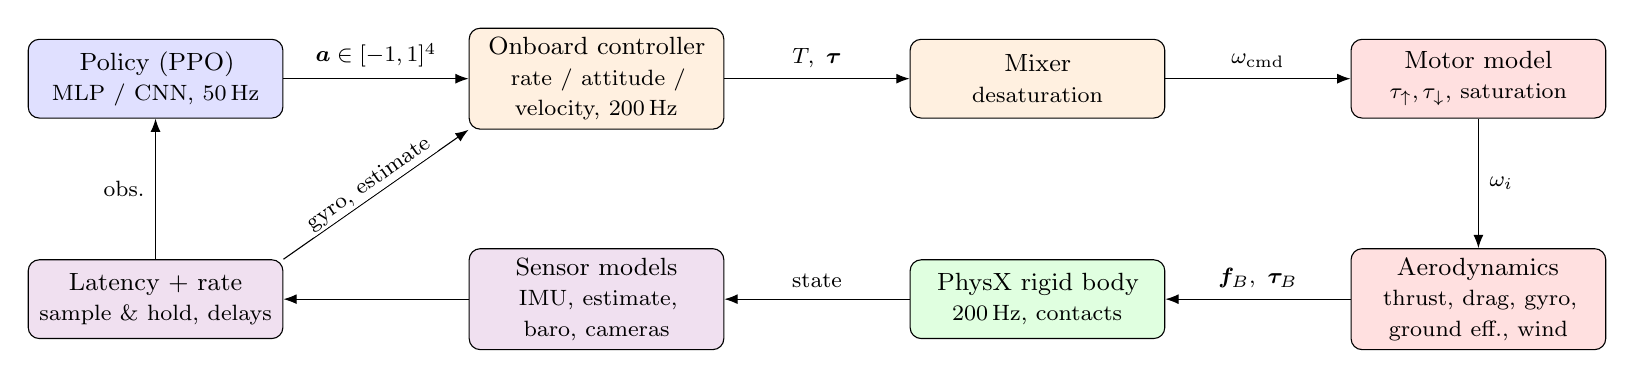
\begin{tikzpicture}[every node/.style={font=\small},
  box/.style={draw, rounded corners, align=center, minimum height=10mm, text width=30mm, fill=#1!12}, box/.default=gray,
  lab/.style={font=\footnotesize, fill=white, inner sep=1pt}]
\node[box=blue]   (pol)  at (0,0)      {Policy (PPO)\\ \footnotesize MLP / CNN, 50\,Hz};
\node[box=orange] (ctl)  at (5.6,0)    {Onboard controller\\ \footnotesize rate / attitude / velocity, 200\,Hz};
\node[box=orange] (mix)  at (11.2,0)    {Mixer\\ \footnotesize desaturation};
\node[box=red]    (mot)  at (16.8,0)   {Motor model\\ \footnotesize $\tau_{\uparrow},\tau_{\downarrow}$, saturation};
\node[box=red]    (aero) at (16.8,-2.8) {Aerodynamics\\ \footnotesize thrust, drag, gyro, ground eff., wind};
\node[box=green]  (phx)  at (11.2,-2.8) {PhysX rigid body\\ \footnotesize 200\,Hz, contacts};
\node[box=violet] (sen)  at (5.6,-2.8) {Sensor models\\ \footnotesize IMU, estimate, baro, cameras};
\node[box=violet] (dly)  at (0,-2.8)   {Latency + rate\\ \footnotesize sample \& hold, delays};
\draw[-Latex] (pol) -- node[lab, above=1mm]{$\vect a\in[-1,1]^4$} (ctl);
\draw[-Latex] (ctl) -- node[lab, above=1mm]{$T,\ \bm\tau$} (mix);
\draw[-Latex] (mix) -- node[lab, above=1mm]{$\omega_{\mathrm{cmd}}$} (mot);
\draw[-Latex] (mot) -- node[lab, right=1mm]{$\omega_i$} (aero);
\draw[-Latex] (aero) -- node[lab, above=1mm]{$\vect f_B,\ \bm\tau_B$} (phx);
\draw[-Latex] (phx) -- node[lab, above=1mm]{state} (sen);
\draw[-Latex] (sen) -- (dly);
\draw[-Latex] (dly) -- node[lab, left=1mm, align=right]{obs.} (pol);
\draw[-Latex] (dly.north east) -- node[lab, sloped, above]{gyro, estimate} (ctl.south west);
\end{tikzpicture}}
\caption{Per-step data flow. Orange, red and violet blocks belong to the framework-agnostic PyTorch core
(\texttt{quadsim.core}) and are unit-tested without Isaac Sim; the green block is PhysX (Isaac Sim). Rendering
(RTX cameras) is an alternative source of image observations.}
\label{fig:arch}
\end{figure}

The code base is layered (\cref{fig:arch}):
\begin{itemize}
\item \texttt{quadsim.core} (pure PyTorch): parameters, motor/aerodynamic model, reference integrators, controllers,
sensor and disturbance models, analytic ray casting (PyTorch and NVIDIA Warp kernels).
\item \texttt{quadsim.isaac}: procedural USD quadrotor (explicit \texttt{MassAPI}: mass, inertia and CoM are written
from the parameters, not derived from geometry) and version-gated runtime patches for upstream issues.
\item \texttt{quadsim.tasks}: Isaac Lab \texttt{DirectRLEnv} base environment and tasks, PPO configurations and
classical baselines that act through the same action interface.
\item \texttt{quadsim.rl}, \texttt{quadsim.data}, \texttt{quadsim.deploy}: networks and policy I/O, HDF5 recording,
export and the NumPy deployment interface.
\end{itemize}
Isaac Lab itself is not modified; it is installed from a pinned tag into \texttt{third\_party/}.

\paragraph{Simulation timeline.} Physics runs at \SI{200}{Hz}, the policy at \SI{50}{Hz} (decimation 4). Within each
physics step: sensors are sampled; the delayed policy command is passed to the onboard controller (which uses the
\emph{noisy} gyro and state estimate); the mixer produces rotor-speed commands; motor states are advanced exactly;
the aerodynamic wrench is evaluated and written to PhysX through Isaac Lab's wrench composer (body frame); PhysX
integrates the rigid body and contacts.

%==========================================================================================
\section{Mathematical models}
\subsection{Frames and rigid-body dynamics}
The world frame $W$ is $z$-up (ENU-like), the body frame $B$ is FLU, and $\vect q\in S^3$ (scalar first) rotates
$B$ into $W$ with rotation matrix $\vect R(\vect q)$. With mass $m$ and principal inertia
$\vect J=\mathrm{diag}(J_x,J_y,J_z)$,
\begin{align}
\dot{\vect p} &= \vect v, &
\dot{\vect v} &= \tfrac{1}{m}\vect R\,\vect f_B + \vect g + \tfrac{1}{m}\vect f^{\mathrm{ext}}_W,\\
\dot{\vect q} &= \tfrac12\,\vect q\otimes\begin{bmatrix}0\\ \bm\omega\end{bmatrix}, &
\vect J\dot{\bm\omega} &= \bm\tau_B - \bm\omega\times\vect J\bm\omega ,
\end{align}
with $\vect g=(0,0,-9.81)$. PhysX integrates these equations with a symplectic (semi-implicit) Euler scheme and
gyroscopic forces enabled; the reference integrator offers RK4 and the same semi-implicit scheme.

\subsection{Rotors and motors}
Rotor $i$ at lever arm $\vect r_i$ (relative to the CoM) with spin $s_i=+1$ (CCW) or $-1$ spins at $\omega_i$:
\begin{equation}
\dot\omega_i = \frac{\omega_{\mathrm{cmd},i}-\omega_i}{\tau_i},\qquad
\tau_i=\begin{cases}\tau_\uparrow & \omega_{\mathrm{cmd},i}\ge\omega_i\\ \tau_\downarrow & \text{otherwise}\end{cases},
\qquad \omega_{\mathrm{cmd},i}\in[\omega_{\min},\omega_{\max}],
\end{equation}
discretized exactly under zero-order hold: $\omega_i^{+}=\omega_{\mathrm{cmd}}+(\omega_i-\omega_{\mathrm{cmd}})e^{-\Delta t/\tau_i}$.
Thrust and reaction torque are $T_i=k_f\,\omega_i^2\,g_e(h_i)$ and
$Q_i=-s_i\,(k_m T_i + J_r\dot\omega_i)$, the latter including the spin-up reaction of the rotor inertia $J_r$.

\subsection{Aerodynamics}
With air-relative velocity $\vect v_{\mathrm{rel}}=\vect v_B-\vect w_B$ (wind $\vect w$) and its component
$\vect v_{\perp,i}$ orthogonal to the rotor axis at the hub ($\vect v_{\mathrm{rel}}+\bm\omega\times\vect r_i$),
\begin{align}
\vect f_{\mathrm{rd},i} &= -c_{\mathrm{rd}}\,\omega_i\,\vect v_{\perp,i} \quad\text{(blade flapping / induced drag)},&
\vect m_{\mathrm{rm},i} &= -c_{\mathrm{rm}}\,s_i\,\omega_i\,\vect v_{\perp,i},\\
\vect f_{\mathrm{body}} &= -\vect D_1\vect v_{\mathrm{rel}} - \vect D_2\,|\vect v_{\mathrm{rel}}|\odot\vect v_{\mathrm{rel}}, &
\bm\tau_{\mathrm{gyr}} &= -\bm\omega\times\textstyle\sum_i J_r s_i\omega_i\,\vect e_z,
\end{align}
and the in-ground-effect gain of Cheeseman and Bennett, $g_e(h)=\left(1-(R/4h)^2\right)^{-1}$, capped at
$h\ge R/2$. The total body wrench is
\begin{equation}
\vect f_B=\sum_i\big(T_i\vect e_z+\vect f_{\mathrm{rd},i}\big)+\vect f_{\mathrm{body}},\quad
\bm\tau_B=\sum_i\big[\vect r_i\times(T_i\vect e_z+\vect f_{\mathrm{rd},i})+\vect m_{\mathrm{rm},i}+Q_i\vect e_z\big]+\bm\tau_{\mathrm{gyr}} .
\end{equation}
The X500 preset uses the PX4 Gazebo values ($k_f=8.549\times10^{-6}$, $k_m=0.016$, $\tau_\uparrow=12.5$\,ms,
$\tau_\downarrow=25$\,ms, $\omega_{\max}=1000$\,rad/s, $c_{\mathrm{rd}}=8.06\times10^{-5}$); its composite mass and
inertia (base + rotors, parallel-axis theorem) are $m=2.064$\,kg, $\vect J=\mathrm{diag}(0.0239,0.0239,0.0440)$\,kg\,m$^2$,
hover speed $769.6$\,rad/s and thrust-to-weight 1.69. Body drag coefficients are engineering estimates (not identified).

\subsection{Wind and disturbances}
Wind is $\vect w=\bar{\vect w}+\vect w_{\mathrm{t}}+\vect w_{\mathrm{g}}$: a per-episode mean, Gauss--Markov turbulence
$\vect w_{\mathrm t}^{+}=a\vect w_{\mathrm t}+\sigma\sqrt{1-a^2}\,\bm\eta$ with $a=e^{-\Delta t/\tau_w}$ (exact
discretization of a Dryden-like first-order process with stationary standard deviation $\sigma$) and discrete
$1-\cos$ gusts (MIL-F-8785C shape) with Poisson arrivals. Push disturbances apply random finite-duration forces.

\subsection{Control allocation and classical controllers}
The allocation $[F_z,\tau_x,\tau_y,\tau_z]^\top=\vect A\vect T$ with rows $(1,\,y_i,\,-x_i,\,-s_ik_m)$ is inverted with
PX4-style sequential desaturation: roll/pitch are scaled only if their spread exceeds the actuator range, the
collective is shifted to preserve roll/pitch authority, and yaw is added with the largest feasible scale.
The onboard rate controller is $\bm\tau=\vect J(\vect K_p\vect e_\omega+\vect K_i\!\int\!\vect e_\omega-\vect K_d\dot{\bm\omega}_f)+\bm\omega\times\vect J\bm\omega$
(derivative on the filtered measurement), the attitude controller is a quaternion P law on the rotation vector
of $\vect q^{-1}\otimes\vect q_{\mathrm{sp}}$, and the position controller is a P--PI cascade producing a thrust vector
with acceleration and tilt limits. The geometric baseline uses Lee et al.'s SE(3) law~\cite{lee2010geometric}
$\vect f=m(-\vect K_x\vect e_x-\vect K_v\vect e_v+g\vect e_3+\ddot{\vect p}_d)$.

\subsection{Sensor models}
\textbf{IMU:} $\tilde{\bm\omega}=(\vect I+\vect M_g)\bm\omega+\vect b_g+\vect n_g$,
$\tilde{\vect a}=(\vect I+\vect M_a)\vect R^\top(\dot{\vect v}-\vect g)+\vect b_a+\vect n_a$, where the specific force
is obtained by finite differences of the PhysX velocity (exact for the symplectic scheme), white noise has density
$\sigma_c$ (discrete std $\sigma_c/\sqrt{\Delta t_s}$), and biases are a per-episode turn-on value plus a Gauss--Markov drift
with random-walk intensity $\sigma_{rw}$ (stationary std $\sigma_{rw}\sqrt{\tau/2}$). Default values are the PX4/rotors
SITL IMU parameters. Measurements are sampled and held at the sensor rate and pass a per-episode random delay.
\textbf{State estimate:} $\hat{\vect p}=\vect p+\vect b_p+\vect x_p+\vect d_p+\vect n_p$,
$\hat{\vect v}=\vect v+\vect x_v+\vect n_v$, attitude with a multiplicative rotation-vector error, all delayed by a
per-episode latency; $\vect b_p\sim\mathcal N(0,\mathrm{diag}\,\bm\sigma_b^2)$ is a per-flight bias, $\vect x_p,\vect x_v$
are first-order Gauss--Markov processes ($\dot{\vect x}=-\vect x/\tau+\sigma\sqrt{2/\tau}\,\vect w$, exact
discretization $\vect x_{k+1}=a\vect x_k+\sigma\sqrt{1-a^2}\,\bm\xi_k$, $a=e^{-\Delta t/\tau}$), $\vect d_p$ a random walk and
$\vect n$ white noise. The v0 tasks use only the white and random-walk terms (EKF/VIO/mocap-like); the parameters of
the correlated terms of the v1 tasks were identified from PX4 EKF2 in SITL (\cref{sec:sitl-est}). \textbf{Barometer:} ISA conversion with noise and Gauss--Markov
bias. \textbf{Depth camera:} distance-to-image-plane with stereo-like noise $\sigma(z)=\sigma_0+kz^2$, quantization,
per-pixel dropouts, minimum/maximum range; no-return pixels read as maximum range. \textbf{Analytic ray casting:}
exact ray--plane, ray--finite-cylinder (side and cap) and ray--oriented-box intersections, implemented in PyTorch
and as an NVIDIA Warp kernel with $O(N R)$ memory.

%==========================================================================================
\section{Reinforcement-learning environments}
\subsection{Observation and action design}
The \texttt{policy} observation contains only quantities available onboard: estimated body-frame velocity, the first
two columns of the estimated rotation matrix (continuous attitude representation), gyro rates, the previous action
and task information expressed in the estimated body frame. The \texttt{critic} additionally receives the true state,
normalized rotor speeds, wind, disturbance force, and normalized domain-randomization parameters
(asymmetric actor-critic~\cite{pinto2018asymmetric}). Four action interfaces are available: individual rotor thrusts,
collective thrust and body rates (CTBR, the default for agile tasks following~\cite{kaufmann2022benchmark}),
collective thrust and attitude, and velocity commands (default for navigation, matching PX4 offboard velocity control).

\subsection{Tasks and rewards}
All rewards are integrated over the policy step $\Delta t$; crashes (ground contact, excessive tilt, velocity, distance,
or obstacle collision) terminate the episode with a penalty.
\begin{itemize}
\item \textbf{Hover/recovery}: initial states up to $\pm1.5$\,m offset, $57^\circ$ tilt, \SI{1.5}{m/s},
\SI{3}{rad/s}; reward $1-\tanh(\|e_p\|/0.8)+0.5\,e^{-(\|e_p\|/0.1)^2}+0.2\cos^2(e_\psi/2)$ minus velocity,
body-rate and action-rate penalties.
\item \textbf{Tracking}: references $\vect p_d(t)=\vect c+\sum_k\vect A_k\sin(\bm\omega_kt+\bm\phi_k)$ covering circles,
figure-eights and random smooth curves (peak speed $\le\SI{4}{m/s}$); the policy observes the reference at
$t+\{0,0.1,0.2,0.4,0.6,1.0\}$\,s.
\item \textbf{Waypoints}: five random waypoints (separation $\ge1.5$\,m); progress reward
$\|\vect p-\vect w\|_{t-1}-\|\vect p-\vect w\|_t$, reach bonus, time penalty.
\item \textbf{Obstacle navigation}: up to 24 kinematic cylinders ($r\in[0.15,0.45]$\,m) rejection-sampled with a
minimum gap of \SI{0.9}{m}, goal $11$--$12$\,m ahead; progress, goal, heading-alignment (camera looks where the vehicle
flies), altitude-band and proximity terms. A curriculum increases the maximum obstacle count from 8 to 24 when the
running success rate exceeds 70\,\%. Observation variants: 32-ray range ring, analytic depth (64$\times$48,
HFOV $87^\circ$), RTX depth, RGB, RGB-D.
\end{itemize}

\subsection{Domain randomization}\label{sec:dr}
Startup (written to PhysX): mass $\times[0.9,1.1]$, inertia $\times[0.85,1.15]$ per axis, CoM offset $\pm$\SI{1}{cm}.
Per episode (model side): $k_f\times[0.9,1.1]$ per rotor, $k_m\times[0.85,1.15]$, motor time constants
$\times[0.7,1.6]$, $\omega_{\max}\times[0.92,1]$ (battery sag), drag $\times[0.5,1.5]$, payload $-5\ldots+10\,\%$ of weight,
sensor-noise scale $\times[0.5,1.5]$, action delay 0--2 and estimator delay 0--2 physics steps.
The \emph{v1} tasks (\texttt{Quadsim-\{Hover,Track,Waypoint\}-v1}) add the corrections found in the PX4 SITL
cross-check (\cref{sec:sitl}): the EKF-like estimate model, action and estimator delays of 0--4 steps (\SIrange{0}{20}{ms}),
noise scale $\times[0.5,2]$, a per-episode rate-PID gain scale $\times[0.6,1.4]$ and a thrust-map gain around hover,
$C=C_h+g\,(C_{\mathrm{cmd}}-C_h)$ with $g\in[0.8,1.7]$, which represents a thrust-curve or calibration error of the
deployed thrust mapping. \texttt{Quadsim-Hover-v2} additionally restores the v0 white-noise level and penalizes the change
of the collective command (\cref{sec:v1}).

\subsection{Learning algorithm}
PPO~\cite{schulman2017ppo} (rsl\_rl 3.1.2) with GAE ($\gamma=0.99,\lambda=0.95$), adaptive learning rate (KL target
0.01), 32 steps per environment, empirical observation normalization. State policies: actor MLP 256--256--128,
critic 512--256--128 (ELU). Vision policies: a 3-layer CNN encoder (32/64/64 channels) to a 128-d feature, fused with
the normalized state in a 256--128 actor; the critic is a state-only MLP on privileged inputs.

%==========================================================================================
\section{Validation and experiments}
\Cref{tab:milestones} summarizes the acceptance status of every milestone; the subsections give the evidence.

\begin{table}[h]
\centering\small
\begin{tabularx}{\linewidth}{lXl}
\toprule
Milestone & Acceptance criterion (executed) & Status\\\midrule
M1 Isaac Sim/Lab & headless GPU boot; PhysX free fall vs symplectic Euler $<\SI{1}{mm}$ (got \SI{9.5e-7}{m}) & \ok\\
M2 Dynamics & unit tests (all modules); PhysX vs reference $<\SI{1}{cm}$/1.5\,s; inertia exact; motor/yaw models $<3\,\%$ & \ok\\
M3 Sensors, recording, visualization & sensor statistics; rendered vs analytic depth (median $<\SI{2}{cm}$); HDF5 round trip; GUI and video & \ok\\
M4 State-based RL & training completes with checkpoints; evaluated vs classical baselines & \ok\\
M5 Vision RL & depth policy trained and evaluated (incl.\ rendered depth); RGB/RGB-D pipelines execute & \ok$^*$\\
M6 DR \& Sim-to-Real interfaces & DR ablation; ONNX = PyTorch to $10^{-5}$; deployment-in-the-loop; ROS 2/PX4 bridge & \ok$^\dagger$\\
M7 Docker, benchmark, docs & container runs tests + GPU smoke test; benchmark table; README; report & \ok\\
PX4 SITL & policies fly PX4 v1.16 SITL as offboard controllers; quadsim-vs-SITL comparison of hover, steps, tracking,
waypoints, navigation; bridge safety gating verified & \ok$^\ddagger$\\
\bottomrule
\end{tabularx}
\caption{Milestone acceptance summary. $^*$Criteria met; the depth policy's success (61--67\,\%) is moderate and
no RGB(-D) policy performance is claimed. $^\dagger$DR showed no significant success gain on hover; the bridge was
validated in PX4 SITL afterwards. $^\ddagger$Hover, tracking and waypoint transfer at the control level; the velocity
navigation policy needs a matched velocity loop (\cref{sec:sitl}).}
\label{tab:milestones}
\end{table}

\subsection{M1: simulator foundation}
Sixty-four rigid bodies in free fall for \SI{0.5}{s} at $\Delta t=\SI{2.5}{ms}$ end at
$|z-z_{\mathrm{symplectic}}|=\SI{9.5e-7}{m}$ (float32 resolution) and $|z-z_{\mathrm{analytic}}|=\SI{6.1}{mm}$, which is exactly the
expected first-order bias $g\,t\,\Delta t/2$; this identifies PhysX's integrator as symplectic Euler, which the reference
simulator reproduces. The same test passes inside the Docker container.

\subsection{M2: quadrotor dynamics}
Unit tests (CPU, no simulator) verify quaternion algebra, FLU sign conventions of roll/pitch/yaw torques, the exact
motor step response ($63.2\,\%$ after $\tau$, separate rise/fall constants, discretization invariance), rotor and body drag,
ground effect and gyroscopic torque, analytic free fall, constant-torque yaw, conservation of angular momentum and energy
for a tumbling body (Dzhanibekov effect), first-order convergence of the semi-implicit integrator to RK4, closed-loop
position steps with the full cascade ($<\SI{5}{cm}$), recovery of the Crazyflie from $46^\circ$ tilt and
\SI{3.7}{rad/s}, SE(3) circle tracking ($<\SI{10}{cm}$ RMSE), and allocation/desaturation properties.
\Cref{tab:m2} lists the Isaac Sim integration tests; \cref{fig:m2} shows the open-loop comparison.

\begin{table}[h]\centering\small
\resizebox{\linewidth}{!}{\begin{tabular}{lccc}\toprule
Test & X500 & Crazyflie & Criterion\\\midrule
PhysX mass / inertia rel. error & 0e+00 / 0e+00 & 0e+00 / 0e+00 & $<10^{-4}$\\
Hover altitude drift over 2\,s [mm] & 0.00 & 0.00 & $<5$\\
Thrust step: accel. RMS err / peak & 0.019\,\% & 0.026\,\% & $<2\,\%$\\
Yaw accel. vs $\tau_z/J_z$ & 0.0036\,\% & 0.0077\,\% & $<3\,\%$\\
Open loop 1.5\,s, pos. err vs semi-implicit ref. [mm] & 0.40 & 2.07 & $<10$\\
Open loop, att. err vs semi-implicit ref. [deg] & 0.006 & 0.066 & $<0.5$\\
Open loop, pos. err vs RK4 ref. [mm] (PhysX discretization) & 3.3 & 8.9 & info\\
Closed-loop velocity cascade, PhysX vs ref. [mm] & 12.3 & 9.2 & $<30$\\
\bottomrule\end{tabular}
}
\caption{PhysX integration of the quadrotor model vs analytic models and the independent reference integrator
(\texttt{scripts/validation/m2\_dynamics\_validation.py}). Sensor noise, latency and randomization disabled.}
\label{tab:m2}
\end{table}
\begin{figure}[h]\centering
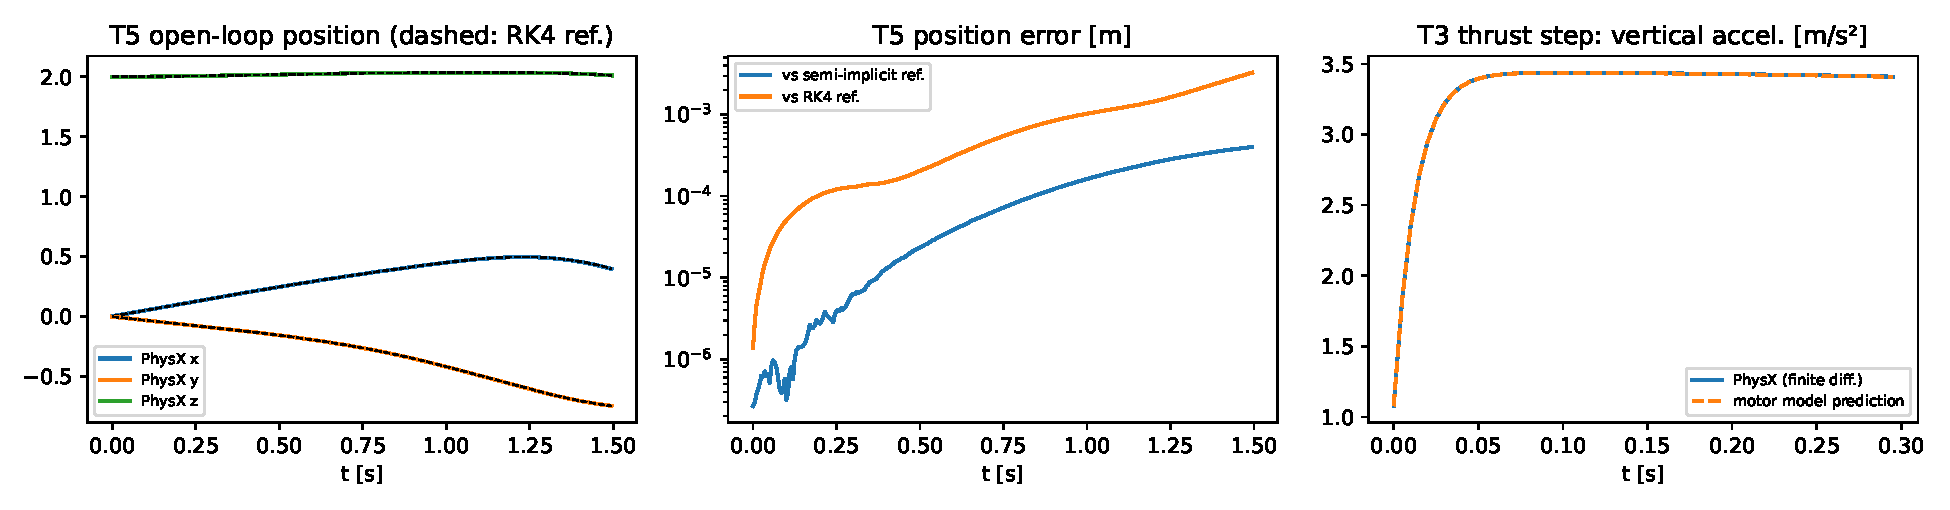
\includegraphics[width=\linewidth]{m2_dynamics_x500.pdf}
\caption{X500: open-loop multisine rotor excitation (left), position error of PhysX vs the reference integrator (middle;
semi-implicit reference = same discretization, RK4 = integration error of PhysX at \SI{200}{Hz}) and thrust-step
response (right).}
\label{fig:m2}
\end{figure}

\subsection{M3: sensors, recording and visualization}
Statistical unit tests confirm the IMU white-noise standard deviation at \SI{200}{Hz} ($\sigma_c\sqrt{f}$, within
$5\,\%$), turn-on bias, exact latency, zero specific force in free fall and the correct gravity direction when tilted,
ISA barometric conversion (\SI{100}{m}~$\to$~\SI{100129}{Pa}), Gauss--Markov stationary statistics, depth-noise
statistics, exact ray--primitive intersections and agreement of the Warp ray-casting kernel with the PyTorch
implementation. A recording plot revealed a bug (no-return depth pixels received $\sigma\propto z^2$ noise); it was fixed
and a regression test added.

\textbf{Rendered vs analytic depth.} For 64 random poses among 24 obstacles (96$\times$72, HFOV $87^\circ$, noise off),
RTX-rendered and analytic depth agree as in \cref{tab:depth}. Residuals concentrate on silhouette pixels (anti-aliasing)
and cylinder tessellation. The comparison also exposed that the initial camera mount saw the X500's front rotor discs
(3\,\% of the image); the default mount was moved to $(0.15,0,-0.06)$\,m, which has no self-occlusion at zero pitch.

\begin{table}[h]\centering\small
\begin{tabular}{lccccc}\toprule
Camera pitch & median [mm] & p90 [cm] & hit/miss agree & self-occl. & pixels\\\midrule
0$^\circ$ & 7.2 & 2.4 & 99.6\,\% & 0.0\,\% & 337361\\
15$^\circ$ & 9.0 & 2.3 & 99.5\,\% & 5.6\,\% & 254392\\
\bottomrule\end{tabular}

\caption{RTX TiledCamera depth vs analytic ray-cast depth (\texttt{scripts/validation/m3\_depth\_consistency.py}).
Self-occluded pixels (vehicle rotors, rendered $<\SI{0.4}{m}$, analytic $>\SI{0.45}{m}$) are excluded from the error
metrics and reported separately.}
\label{tab:depth}
\end{table}
\begin{figure}[h]\centering
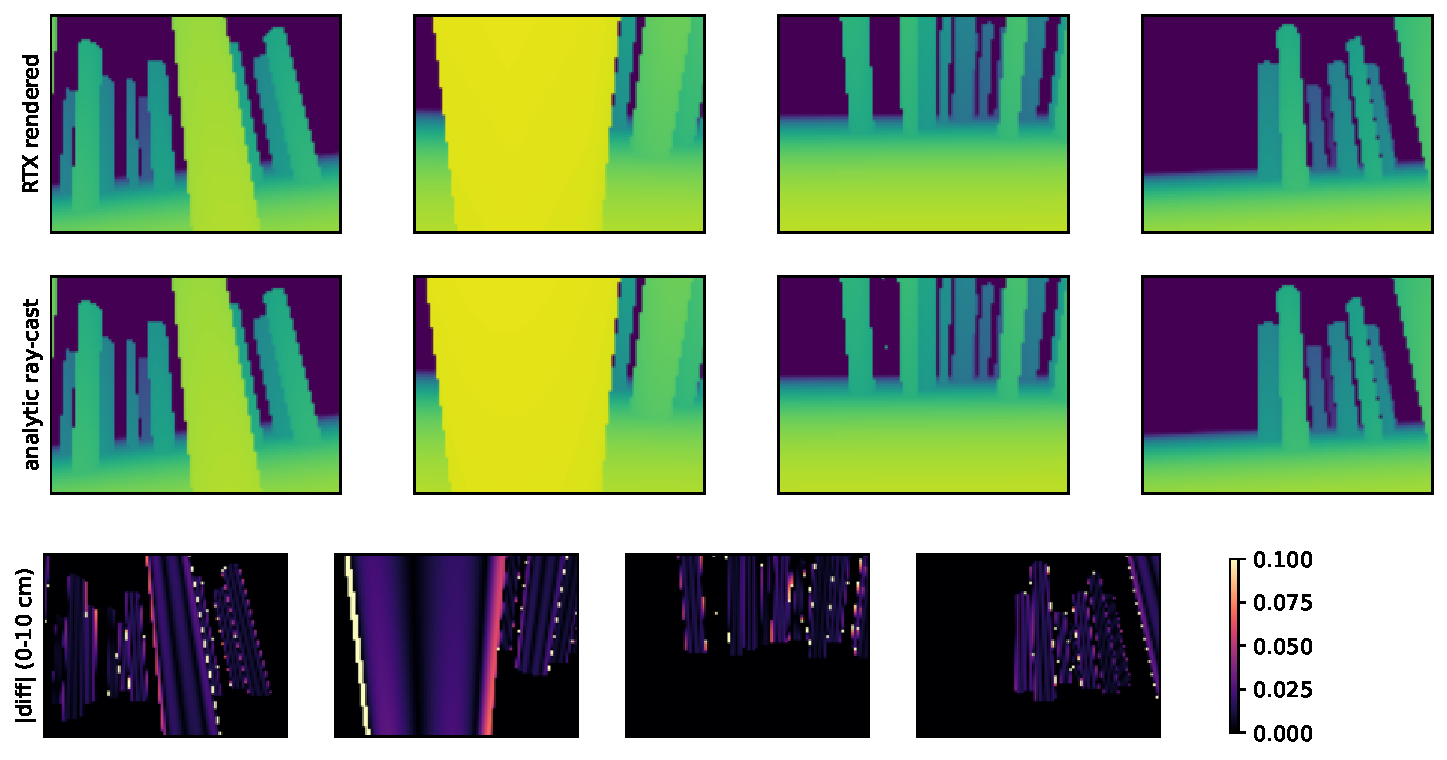
\includegraphics[width=\linewidth]{m3_depth_consistency_pitch0.pdf}
\caption{Rendered depth (top), analytic ray-cast depth (middle) and absolute difference clipped at \SI{10}{cm} (bottom).}
\end{figure}

\textbf{Recording.} The synchronized HDF5 recorder was verified by round trips for a state task (tracking, SE(3)
baseline) and a rendered-depth task (navigation, potential-field baseline): dataset shapes, monotonic timestamps with
constant $\Delta t$, exact equality of the last sample with the live simulator, and the embedded configuration.
\textbf{Visualization.} Headless MP4 recording and the interactive GUI viewer (chase camera, target and reference markers)
work after patching an upstream Isaac Lab issue (\cref{sec:patch}).

\subsubsection{Upstream issue found and patched}\label{sec:patch}
With any rendered viewport (GUI, \texttt{--video}), every RigidObject failed to initialize with
``Failed to get rigid body transforms from backend'' --- reproduced with a plain Isaac Lab cuboid. Cause:
\texttt{WrenchComposer.\_\_init\_\_} uses \texttt{hasattr(asset.data, "body\_link\_pos\_w")}; \texttt{hasattr}
evaluates the property, which queries PhysX before its GPU buffers exist during the PLAY callback, and the raised
\texttt{Exception} is not an \texttt{AttributeError}. quadsim applies a version-gated patch that checks the attribute
on the class (no PhysX query), leaving Isaac Lab's sources untouched. Isaac Lab's viewport chase camera has a similar
start-up read, which the viewer avoids by enabling asset following only after the first reset.

\subsection{M4: state-based reinforcement learning}
All policies use CTBR actions at \SI{50}{Hz}, the full randomization of \cref{sec:dr}, sensor noise and latency.
Evaluation uses the deterministic policy and identical seeds (hence identical initial states and randomization) for all
controllers; $\pm$ denotes a 95\,\% confidence interval of the mean.

\textbf{Hover and recovery.} Training: 4096 environments, 600 PPO iterations (\SI{79}{M} transitions, $\approx$\SI{10}{min}
on the RTX~5060). Success requires $\|e_p\|<\SI{10}{cm}$ and $\|v\|<\SI{0.2}{m/s}$ at the end of the \SI{8}{s} episode.
The policy also generalizes to wind (0--3\,m/s mean, turbulence, gusts) and push disturbances that were \emph{not}
present during training (\cref{tab:hover}). The policy's yaw accuracy ($4.4^\circ$) is worse than the baseline's because of
the weak yaw reward weight.
\begin{table}[h]\centering\small
\resizebox{\linewidth}{!}{\begin{tabular}{llccccc}\toprule
Condition & Controller & success [\%] & crash [\%] & final pos. err [cm] & final yaw err [deg] & episodes\\\midrule
nominal & PPO (ours) & 99.9 $\pm$ 0.2 & 0.0 $\pm$ 0.0 & 1.26 $\pm$ 0.04 & 4.4 $\pm$ 0.2 & 1000\\
nominal & Cascade PID & 90.3 $\pm$ 1.8 & 0.6 $\pm$ 0.5 & 6.28 $\pm$ 0.95 & 1.5 $\pm$ 0.3 & 1000\\
\midrule
wind + pushes & PPO (ours) & 97.2 $\pm$ 1.0 & 0.0 $\pm$ 0.0 & 2.71 $\pm$ 0.11 & 4.6 $\pm$ 0.2 & 1000\\
wind + pushes & Cascade PID & 80.8 $\pm$ 2.4 & 0.5 $\pm$ 0.4 & 7.60 $\pm$ 0.84 & 1.5 $\pm$ 0.3 & 1000\\
\bottomrule\end{tabular}
}
\caption{Hover/recovery from up to $57^\circ$ tilt, \SI{3}{rad/s}, \SI{1.5}{m/s} and \SI{1.5}{m} offset (1000 episodes per row).}
\label{tab:hover}
\end{table}

\textbf{Trajectory tracking.} Training: 4096 environments, 1500 iterations (\SI{197}{M} transitions). The aggressive
reference set contains accelerations up to $\approx$\SI{15}{m/s^2}, partly beyond the X500's sustainable
\SI{13}{m/s^2} (thrust-to-weight 1.69) and beyond the baselines' tilt limits; the moderate set ($\le$\SI{2}{m/s},
$\le$\SI{0.35}{Hz}) is feasible for all controllers. The first SE(3) baseline, which mapped Lee's torque-level attitude
law onto rate set-points at the \SI{50}{Hz} policy rate, was unstable (53\,\% crashes, row $\dagger$); the redesigned
baseline uses Lee's position law with the onboard attitude/rate loops.
\begin{table}[h]\centering\small
\resizebox{\linewidth}{!}{\begin{tabular}{llcccc}\toprule
Reference set & Controller & RMSE [cm] & max err [cm] & crash [\%] & episodes\\\midrule
aggressive ($\le$4\,m/s) & PPO (ours) & 12.6 $\pm$ 1.5 & 40.6 $\pm$ 3.0 & 0.2 $\pm$ 0.4 & 500\\
aggressive ($\le$4\,m/s) & Cascade PID & 46.6 $\pm$ 3.7 & 104.0 $\pm$ 7.3 & 3.0 $\pm$ 1.5 & 500\\
aggressive ($\le$4\,m/s) & SE(3) geometric & 49.0 $\pm$ 3.8 & 97.6 $\pm$ 6.8 & 3.2 $\pm$ 1.5 & 500\\
aggressive ($\le$4\,m/s) & SE(3) v1 (torque-level @50\,Hz)$^\dagger$ & 114.2 $\pm$ 5.0 & 221.8 $\pm$ 9.0 & 53.2 $\pm$ 4.4 & 500\\
\midrule
moderate ($\le$2\,m/s) & PPO (ours) & 5.8 $\pm$ 0.2 & 29.0 $\pm$ 0.8 & 0.0 $\pm$ 0.0 & 500\\
moderate ($\le$2\,m/s) & Cascade PID & 17.6 $\pm$ 1.4 & 50.6 $\pm$ 3.8 & 0.2 $\pm$ 0.4 & 500\\
moderate ($\le$2\,m/s) & SE(3) geometric & 22.7 $\pm$ 1.4 & 52.8 $\pm$ 3.8 & 0.2 $\pm$ 0.4 & 500\\
\bottomrule\end{tabular}
}
\caption{Trajectory tracking (500 episodes of \SI{10}{s} per row). Maximum errors include the initial transient
(start offset up to \SI{0.3}{m}).}
\label{tab:track}
\end{table}

\textbf{Waypoint navigation.} Training: 4096 environments, 1500 iterations. Five random waypoints (separation
$\ge\SI{1.5}{m}$, \SI{0.3}{m} acceptance radius) must be passed in order within \SI{15}{s}. The cascade baseline
flies to each waypoint with its velocity limits (\SI{5}{m/s} horizontal), facing the waypoint.
\begin{table}[h]\centering\small
\resizebox{\linewidth}{!}{\begin{tabular}{llccccc}\toprule
Condition & Controller & success [\%] & waypoints [\%] & time [s] & crash [\%] & episodes\\\midrule

\bottomrule\end{tabular}
}
\caption{Waypoint navigation (500 episodes). Time is measured over successful episodes only.}
\label{tab:wp}
\end{table}

\subsection{M5: obstacle-avoidance navigation (range and depth)}
The navigation task is the hardest: up to 24 cylinders in an $8\times8$\,m field with \SI{0.9}{m} minimum surface
gap for a vehicle of \SI{0.35}{m} collision radius, velocity-command actions and a forward-facing camera
($87^\circ$ HFOV) for the depth policy. Evaluation uses the full density (curriculum off, 4--24 active obstacles,
mean $\approx$12).

\textbf{Reward iteration (documented).} The first reward (proximity weight 0.2, collision $-10$, $\gamma=0.99$)
produced a policy that flies at the \SI{3}{m/s} limit and accepts collisions (52.9\,\% success, 46.3\,\% collision):
the proximity term contributed $\approx-0.005$ per episode and the \SI{2}{s} effective horizon favoured speed.
Reward v2 (proximity 2.0, collision $-20$, $\gamma=0.995$, everything else unchanged) was used for both the range and
the depth policies. The classical potential-field baseline (same range ring) rarely collides but gets trapped in
local minima.

\begin{table}[h]\centering\small
\resizebox{\linewidth}{!}{\begin{tabular}{llccccc}\toprule
Policy input / eval & Controller & success [\%] & collision [\%] & time [s] & min clear. [cm] & episodes\\\midrule
range ring (classical) & Potential field & 39.3 $\pm$ 4.0 & 4.4 $\pm$ 1.7 & 9.86 $\pm$ 0.39 & 71 $\pm$ 2 & 570\\
\midrule
range ring, reward v1 & PPO (ours) & 52.9 $\pm$ 4.4 & 46.3 $\pm$ 4.4 & 3.67 $\pm$ 0.06 & 45 $\pm$ 2 & 501\\
\bottomrule\end{tabular}
}
\caption{Obstacle navigation at full density (curriculum off). The depth policy (trained 900 iterations on analytic
depth) is evaluated both on its training sensor and zero-shot on RTX-rendered depth. Minimum clearance is measured
from the vehicle centre to the nearest cylinder surface (collision below \SI{35}{cm}).}
\label{tab:nav}
\end{table}
Findings (\cref{tab:nav}):
\begin{itemize}
\item \textbf{Reward v2} raised the range-ring policy from 57.8 to \textbf{84.4\,\%} success and cut collisions from
42.2 to 15.6\,\% at nearly the same speed (\SI{4.3}{s} to the goal).
\item \textbf{Classical baseline.} The potential field rarely collides (7\,\%) but is trapped in local minima in
53--56\,\% of the episodes and is $2.5\times$ slower (36.6--39.4\,\% success in two runs). An earlier version of
this report gave 49.8 and 39.3\,\% for the two runs and attributed the spread to unpaired episodes; the actual cause
was the evaluator's sampling bias (\cref{sec:review}), which affected the run with two episodes per environment.
\item \textbf{Depth policy.} With the forward-looking camera only ($87^\circ$ HFOV, no memory), the CNN policy reaches
63.8\,\% success on its training sensor, below the $360^\circ$ range policy (84.4\,\%). A plausible but
\emph{unverified} explanation is that a memoryless policy cannot account for obstacles that have left the camera's
field of view; a recurrent policy or a wider camera are the natural next experiments.
\item \textbf{Analytic vs rendered depth.} Evaluated zero-shot with RTX-rendered depth, the depth policy achieves
60.0\,\% success / 39.7\,\% collisions against 63.8 / 35.8\,\% on the analytic depth it was trained on, a
difference within the confidence intervals (no significant degradation). Together with the pixel-level agreement of \cref{tab:depth}, this justifies training
depth policies with the fast analytic sensor (83\,k vs 6.8\,k env-steps/s, \cref{tab:bench}).
\item \textbf{RGB / RGB-D.} The rendered RGB and RGB-D environments, image augmentation and the CNN actor-critic
execute end to end (10-iteration PPO run with 64 environments). No RGB(-D) policy performance is claimed.
\end{itemize}

\begin{figure}[h]\centering
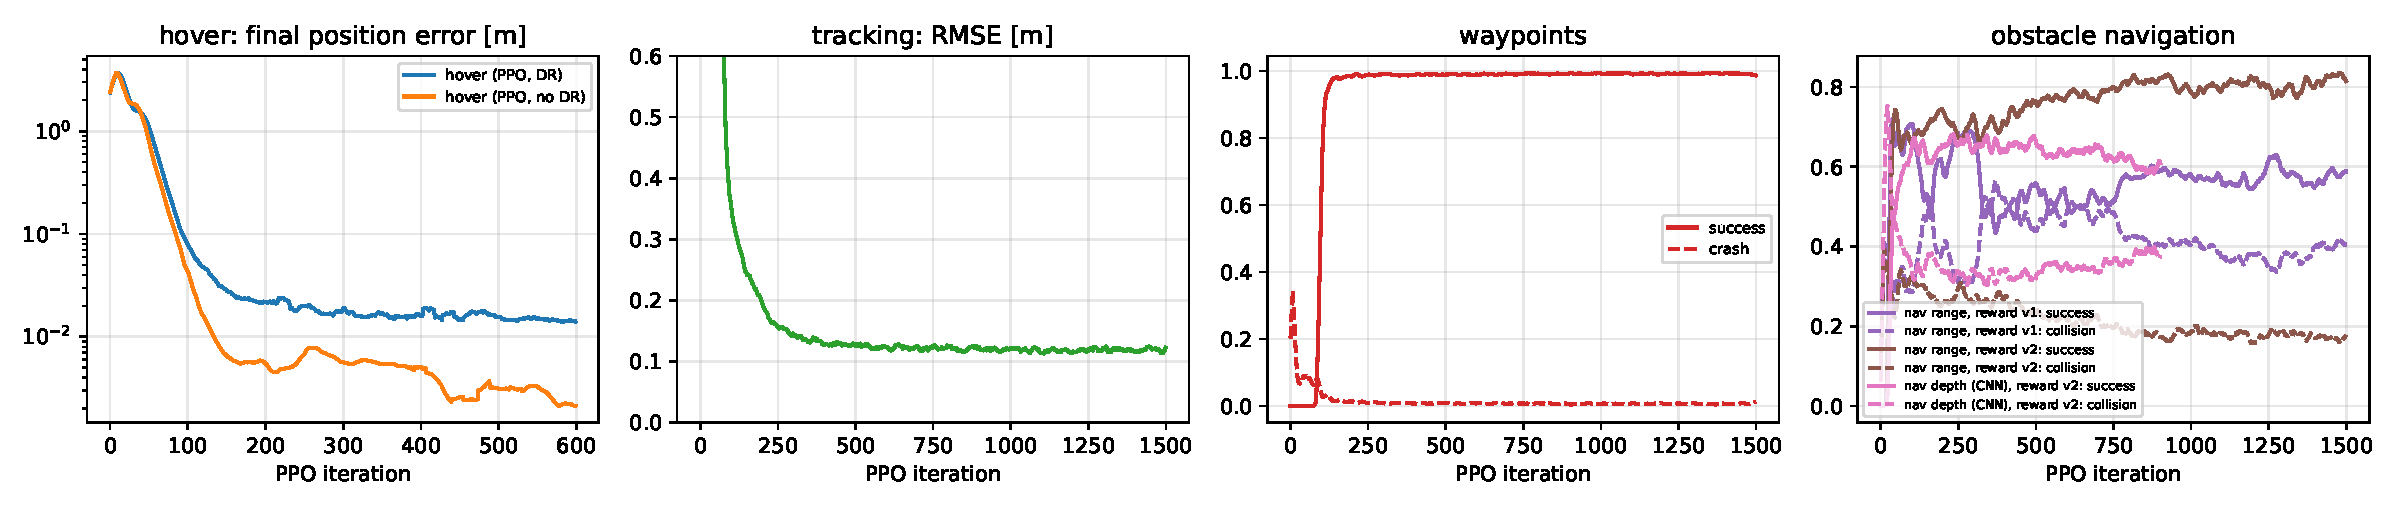
\includegraphics[width=\linewidth]{training_curves.pdf}
\caption{Training curves (episode-end metrics of the stochastic training policy, smoothed). The two hover curves
are each measured on their own training distribution (the no-DR policy trains without noise) and are not directly
comparable; see \cref{tab:dr} for the controlled comparison. Navigation success is measured at the current
curriculum density: the maximum obstacle count rises from 8 to 24, reached at iteration 112 (range v1), 124 (range v2)
and 501 (depth v2); the early decline of the depth curve reflects the densifying forest. The depth run was stopped at
iteration 900 (400 iterations at full density, success flat over the last 300) for compute-time reasons.}
\label{fig:curves}
\end{figure}

\subsection{Domain-randomization ablation}
An identical hover policy was trained without any randomization, sensor noise or latency (\emph{w/o DR}) and compared
with the default policy (\emph{with DR}) under three evaluation conditions: \emph{ideal} (the no-DR training
distribution), \emph{randomized} (the DR training distribution) and \emph{harsh} (outside both training distributions:
mass $\times[0.8,1.25]$, motor time constants $\times[1.5,2.5]$, thrust coefficients $\times[0.8,1.0]$, sensor noise
$\times[1.5,2]$, 10--20\,ms action delay, wind and gusts).
\begin{table}[h]\centering\small
\resizebox{\linewidth}{!}{\begin{tabular}{llccccc}\toprule
Eval. condition & Policy & success [\%] & crash [\%] & final pos. err [cm] & final yaw err [deg] & episodes\\\midrule
ideal & PPO with DR & 100.0 $\pm$ 0.0 & 0.0 $\pm$ 0.0 & 0.22 $\pm$ 0.00 & 3.7 $\pm$ 0.1 & 1000\\
ideal & PPO w/o DR & 100.0 $\pm$ 0.0 & 0.0 $\pm$ 0.0 & 0.28 $\pm$ 0.00 & 9.8 $\pm$ 0.2 & 1000\\
\midrule
randomized & PPO with DR & 99.9 $\pm$ 0.2 & 0.0 $\pm$ 0.0 & 1.26 $\pm$ 0.04 & 4.4 $\pm$ 0.2 & 1000\\
randomized & PPO w/o DR & 99.9 $\pm$ 0.2 & 0.0 $\pm$ 0.0 & 1.92 $\pm$ 0.07 & 10.2 $\pm$ 0.2 & 1000\\
\midrule
harsh & PPO with DR & 78.7 $\pm$ 2.5 & 4.0 $\pm$ 1.2 & 15.93 $\pm$ 2.32 & 19.7 $\pm$ 2.3 & 1000\\
harsh & PPO w/o DR & 78.2 $\pm$ 2.6 & 3.4 $\pm$ 1.1 & 16.78 $\pm$ 2.26 & 21.7 $\pm$ 1.9 & 1000\\
\bottomrule\end{tabular}
}
\caption{DR ablation on the hover task (1000 episodes per row, identical seeds).}
\label{tab:dr}
\end{table}
The DR policy has lower position error in every condition (e.g. \SI{1.26}{} vs \SI{1.92}{cm} under the training
randomization, \SI{15.9}{} vs \SI{16.8}{cm} under harsh conditions), but crash rates (4.0 vs 3.4\,\%) and success
rates (78.7 vs 78.2\,\%) under harsh conditions are within the 95\,\% confidence intervals. We therefore do \emph{not} claim a significant robustness gain from DR for this task. A plausible
explanation is the CTBR interface: the onboard rate loop closes around the (real) gyro and absorbs much of the
inertial and actuator variation, a robustness property reported for CTBR policies in~\cite{kaufmann2022benchmark}.
The yaw error of the DR policy is 2.3--2.7$\times$ lower in the ideal and training conditions but similar under harsh
conditions; with one seed per arm this may be a training-run effect rather than a DR effect. Multi-seed ablations, and ablations with the direct motor interface where
DR is expected to matter more, are planned (\cref{sec:roadmap}).

\subsection{M6: export and deployment pipeline}
The exported ONNX graph (normalizer + actor + clamp) matches PyTorch to $3.6\times10^{-7}$. In the
deployment-in-the-loop test the simulator is flown by the ONNX policy whose observation is rebuilt every step by the
NumPy \texttt{ObservationBuilder} from onboard quantities only. Over 512 hover episodes the maximum observation error is
$9.5\times10^{-7}$, the maximum action error $1.0\times10^{-6}$, and the success rate (99.8\,\%) and final error
(\SI{1.29}{cm}) equal those of the PyTorch policy. Frame conversions to PX4 (NED/FRD) are unit-tested, including the
consistency of a physical body vector through both quaternion conventions.

\subsection{Off-policy baseline: SAC}
To support algorithms beyond PPO, an off-policy Soft Actor-Critic trainer (skrl~1.4.3) runs on the same
environments (\texttt{scripts/rl/train\_sac.py}). On the hover task with 256 environments and 30\,000 vectorized steps
(7.7\,M transitions, 30\,k gradient updates, \SI{21}{min}) the episode return rose monotonically from $-11.2$ to $+1.7$
(still increasing; PPO reaches $\approx 11$ on the same reward). The deterministic policy never crashed but ended
\SI{1.13}{m} from the target on average (0\,\% success over 1024 episodes). SAC is therefore \emph{executing and
learning} but \emph{not competitive} within this budget; a higher update-to-data ratio and tuning are required.
This baseline is superseded by the framework's GPU-native SAC/TD3, which reach 99.9 and 99.6\,\% hover success
(\cref{sec:framework}, \cref{tab:fw_offpolicy}).

\subsection{M7: throughput, memory and containerization}
\Cref{tab:bench} lists environment-stepping throughput (no learning) on the idle RTX~5060 (8\,GB); VRAM is the whole
process including Isaac Sim. State-based tasks scale almost linearly up to 8192 environments
(\SI{0.44}{M}~env-steps/s, \SI{1.76}{M} physics steps/s at \SI{200}{Hz}). Analytic depth (Warp kernel, 3072 rays per
environment) costs only $\approx$1.6$\times$ relative to the state task at 2048 environments, whereas RTX-rendered
cameras are limited to a few thousand env-steps/s. End-to-end training throughput (with PPO updates) was
$\approx$190\,k (hover, 4096 envs), 117\,k (range navigation) and 16\,k env-steps/s (depth CNN, 2048 envs).
\begin{table}[h]\centering\small
\begin{tabular}{lrrrr}\toprule
Task & envs & k env-steps/s & ms / step & VRAM [GB]\\\midrule
\texttt{Hover-v0} & 256 & 16.1 & 15.92 & 2.27\\
\texttt{Hover-v0} & 1024 & 63.0 & 16.26 & 2.96\\
\texttt{Hover-v0} & 4096 & 237.0 & 17.29 & 3.72\\
\texttt{Hover-v0} & 8192 & 438.9 & 18.66 & 3.86\\
\texttt{Nav-Depth-v0} & 256 & 14.5 & 17.67 & 2.33\\
\texttt{Nav-Depth-v0} & 1024 & 52.5 & 19.51 & 3.24\\
\texttt{Nav-Depth-v0} & 2048 & 83.1 & 24.65 & 4.41\\
\texttt{Nav-Depth-Render-v0} & 64 & 2.1 & 29.85 & 4.17\\
\texttt{Nav-Depth-Render-v0} & 128 & 3.8 & 33.77 & 4.85\\
\texttt{Nav-Depth-Render-v0} & 256 & 6.8 & 37.79 & 5.60\\
\texttt{Nav-RGBD-v0} & 64 & 2.1 & 30.66 & 4.19\\
\texttt{Nav-RGBD-v0} & 128 & 3.8 & 33.28 & 4.87\\
\bottomrule\end{tabular}

\caption{Environment throughput and process VRAM (\texttt{scripts/tools/benchmark.py}).}
\label{tab:bench}
\end{table}
The Docker image (\texttt{docker/Dockerfile}, based on \texttt{nvcr.io/nvidia/isaac-lab:2.3.2}) builds, and the
containerized test service passes all unit tests and the Isaac Sim GPU smoke test. Interactive GUI visualization (chase
camera, target/reference markers) and headless MP4 recording of trained policies were verified after the patch of
\cref{sec:patch}.


%==========================================================================================
% PX4 SITL validation (included by report.tex)
\section{PX4 SITL validation and sim-to-sim analysis}\label{sec:sitl}
The exported policies were flown as PX4 offboard controllers against PX4~v1.16.2 software-in-the-loop (SITL) with the
Gazebo Harmonic \texttt{x500} model, whose rotor, motor and inertia parameters equal the quadsim X500 preset. SITL
replaces quadsim's rigid-body engine (PhysX $\to$ gz-physics), its onboard controllers (simulated rate PID and velocity
cascade $\to$ PX4 \texttt{mc\_rate\_control}, \texttt{mc\_pos\_control} and the control allocator) and its estimator model
(noise model $\to$ EKF2 fusing simulated IMU, GNSS, barometer and magnetometer), and adds the real deployment software
path (ROS~2 node, uXRCE-DDS, PX4 time synchronization). Differences between the two simulators therefore expose the
assumptions of the training environment that a real flight would also violate. Every experiment is scripted and
re-runnable (\texttt{ros2/px4\_sitl/setup\_px4\_sitl.sh}, \texttt{scripts/sitl/}); all reported numbers are computed by
the same unit-tested functions (\texttt{quadsim.deploy.closed\_loop\_metrics}) for quadsim and SITL.

\subsection{Setup and deployment pipeline}
\begin{figure}[h]\centering
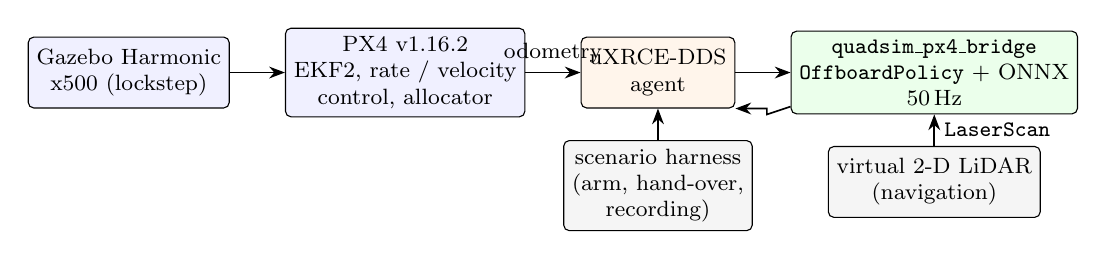
\begin{tikzpicture}[node distance=4mm and 7mm, every node/.style={font=\footnotesize},
  box/.style={draw, rounded corners=2pt, align=center, minimum height=9mm, inner sep=3pt},
  arr/.style={-{Stealth[length=2mm]}, semithick}]
\node[box, fill=blue!6] (gz) {Gazebo Harmonic\\x500 (lockstep)};
\node[box, fill=blue!6, right=of gz] (px4) {PX4 v1.16.2\\EKF2, rate / velocity\\control, allocator};
\node[box, fill=orange!8, right=of px4] (dds) {uXRCE-DDS\\agent};
\node[box, fill=green!8, right=of dds] (bridge) {\texttt{quadsim\_px4\_bridge}\\\texttt{OffboardPolicy} + ONNX\\50\,Hz};
\node[box, fill=gray!8, below=of bridge] (scan) {virtual 2-D LiDAR\\(navigation)};
\node[box, fill=gray!8, below=of dds] (harness) {scenario harness\\(arm, hand-over,\\recording)};
\draw[arr] (gz) -- (px4); \draw[arr] (px4) -- node[above]{odometry} (dds); \draw[arr] (dds) -- (bridge);
\draw[arr] (bridge.south west) ++(0,0.1) -- ++(-0.3,-0.1) |- node[pos=0.25,left]{} (dds.south east);
\draw[arr] (scan) -- node[right]{\texttt{LaserScan}} (bridge);
\draw[arr] (harness) -- (dds);
\end{tikzpicture}
\caption{SITL loop. The bridge receives \texttt{VehicleOdometry} (EKF2, NED/FRD) and publishes
\texttt{OffboardControlMode} plus \texttt{VehicleRatesSetpoint} (CTBR policies) or \texttt{TrajectorySetpoint}
(velocity policies). The harness takes off with PX4, calibrates the thrust map, hands over to the policy, applies the task
and records odometry, simulator ground truth and commands in one time base.}
\label{fig:sitl}
\end{figure}
PX4 runs its EKF2 and controllers unmodified with airframe defaults, except \texttt{NAV\_DLL\_ACT}=0 (no ground
station) and \texttt{EKF2\_GPS\_DELAY}=0 (\cref{sec:sitl-est}). The only change to PX4 is SITL instrumentation that
exports the gz ground truth over DDS for evaluation. The bridge's per-step logic is the ROS-free class
\texttt{quadsim.deploy.offboard.OffboardPolicy}: it rebuilds the training observation of each task (hover goal; tracking
reference $t+\{0,\dots,1\}$\,s generated onboard; waypoint sequence with the training switching rule; navigation goal plus
the 32-ray range ring resampled from any \texttt{LaserScan}) and is checked against the simulator in closed loop
(observation error $\le7.5\times10^{-6}$ for all four tasks, ONNX vs PyTorch success within 3 points; generalized M6
test). A scenario starts with a PX4 take-off and Hold; the goal / reference / course is defined from the current pose and
the policy takes over in OFFBOARD; after the task PX4 takes back control and lands.

\textbf{Thrust map.} PX4 expects a normalized thrust $u\in[0,1]$. For gz \texttt{x500} the ESC maps $u$ to
$\omega=\omega_{\min}+(\omega_{\max}-\omega_{\min})u$ and the thrust is $T=4k_f\omega^2$, i.e.\ $T/T_{\max}=c(u)=(0.15+0.85u)^2$.
The documented calibration (linear map $u=s\,C/T_{\max}$ with $s=u_h/(mg/T_{\max})$ from PX4's hover-thrust estimate $u_h$)
is exact only at hover; there the true local gain exceeds the linear map's by
$\frac{c'(u_h)}{c(u_h)/u_h}=\frac{2\cdot0.85\,u_h}{0.15+0.85u_h}=1.61$ ($u_h=0.7295$). The bridge therefore also supports an
exact curve map $u=c^{-1}(s\,C/T_{\max})$ with $s=c(u_h)/(mg/T_{\max})$ (\texttt{ThrustCurve}); the calibrated
$s=1.0016$ shows that the gz model and the quadsim preset agree on hover thrust within \SI{0.2}{\percent}.

\textbf{Identification tools.} Command$\to$response dynamics are identified from closed-loop flight data by an output-error
fit of a first-order-plus-dead-time model $Y(s)/U(s)=Ke^{-Ls}/(\tau s+1)$ (grid over $L$ and $\tau$, least squares for $K$,
zero-order-held commands); estimator lag by the shift minimizing $\mathrm{E}\|\hat x(t)-x(t-L)\|^2$; limit cycles by the
RMS and Welch-spectrum peak of body rate, collective command and vertical velocity. All are unit-tested on synthetic
signals with known parameters.

\subsection{Defects found by SITL}
\begin{itemize}
\item \textbf{Bridge never commanded.} PX4~1.16 versions some DDS topics (\texttt{VehicleStatus}$\to$
\texttt{/fmu/out/vehicle\_status\_v1}); the original node subscribed to the unversioned name, never saw OFFBOARD and
sent no set-point. Reproduced: PX4 accepted OFFBOARD for \SI{8}{s} without receiving a single set-point and the vehicle
drifted \SI{3.5}{m} on the last attitude-controller command. Topic names are now derived from the message versions.
\item \textbf{Failsafe could never trigger.} PX4 detects offboard loss only from the \texttt{OffboardControlMode}
heartbeat (\texttt{COM\_OF\_LOSS\_T}); the node published it before its stale-odometry and geofence checks. The heartbeat
is now sent only while the node can command; verified: after a geofence violation PX4 left OFFBOARD after
\SI{1.03}{s} and, without RC, landed.
\item Packaging (\texttt{setup.cfg}), a \emph{last-action} input containing never-applied commands before the hand-over,
NaN/frame checks of the odometry.
\item \textbf{Measurement artefacts.} PX4's gz ground-truth velocity and ``angular velocity'' are backward differences
(the latter of Euler angles); truth rates are recomputed by central differences of the ground-truth quaternions. rclpy's
multi-threaded executor dropped $\approx$35\,\% of the messages in the recorder (PX4 itself received every set-point).
\end{itemize}

\subsection{Estimator}\label{sec:sitl-est}
\Cref{tab:sitl-est} summarizes EKF2's error against the gz ground truth. In hover it is dominated by a per-flight bias
(2--4\,cm) and a slow, correlated component (std \SI{1.4}{cm}, correlation time 2--3\,s); the white part is
$\approx$\SI{1}{mm} and the attitude error $\approx$\SI{0.2}{mrad}. quadsim's v0 odometry model is the opposite: mostly
white (\SI{1}{cm} position, \SI{3}{cm/s} velocity, \SI{10}{mrad} attitude). In motion, EKF2 led the truth by
\SI{0.11}{s}: its default GNSS delay compensation (\texttt{EKF2\_GPS\_DELAY}=\SI{110}{ms}, correct for real receivers)
assumes a latency the gz GNSS does not have. Matching it (0\,ms) removed the lead and halved the truth-referenced
tracking error (14$\to$\SI{7}{cm}). These statistics define the EKF-like model of the v1 training distribution.
\begin{table}[h]\centering\small
\begin{tabular}{lc}\toprule
Quantity & PX4 EKF2 in SITL\\\midrule
Per-flight position bias $|\bar e_p|$ (x / y / z) [cm] & 1.8 / 1.8 / 3.9\\
Slow position error ($<$0.5\,Hz) std [cm] & 1.4 / 1.4 / 1.5\\
Slow position error correlation time [s] & 1.7 / 1.9 / 3.2\\
Fast position error std [mm] & 1.3 / 1.5 / 1.1\\
Velocity error std [cm/s] & 0.94 / 1.05 / 0.41\\
Velocity error correlation time [s] & 0.81 / 0.35 / 2.14\\
Roll / pitch error std [mrad] & 0.19 / 0.20\\
Circle flight, \texttt{EKF2\_GPS\_DELAY}=110\,ms: lag x / y [ms], RMS error [cm] & -110 / -99, 12.0\\
Circle flight, \texttt{EKF2\_GPS\_DELAY}=0\,ms: lag x / y [ms], RMS error [cm] & -3 / -1, 6.3\\
\bottomrule\end{tabular}
% 6 hover runs

\caption{PX4 EKF2 error vs gz ground truth (\texttt{scripts/sitl/estimator\_stats.py}, \texttt{docs/results/sitl\_estimator.json}).}
\label{tab:sitl-est}
\end{table}

\subsection{Hover and set-point steps}
The scenario of \cref{tab:sitl-hover} holds the hand-over pose for \SI{30}{s} (RMS over 10--30\,s), then steps the goal by
\SI{1}{m} in $x$ and in $z$; quadsim flies the same schedule with 64 environments starting at the goal.
\begin{table}[h]\centering\small
\resizebox{\linewidth}{!}{\begin{tabular}{lcccc}\toprule
Metric & quadsim nominal & SITL linear map (3) & SITL curve map (4) & SITL linear + geometry fix (2)\\\midrule
Hover RMS error, truth [cm] & 1.59 $\pm$ 0.46 & 4.12 $\pm$ 1.94 & 6.00 $\pm$ 1.11 & 4.71 $\pm$ 1.06\\
Hover RMS error w.r.t. estimate [cm] & 1.88 $\pm$ 0.02 & 1.02 $\pm$ 0.13 & 0.83 $\pm$ 0.04 & 1.01 $\pm$ 0.22\\
Estimate vs truth, hover RMS [cm] & 2.28 $\pm$ 0.31 & 3.84 $\pm$ 2.08 & 5.81 $\pm$ 1.19 & 4.51 $\pm$ 1.08\\
$x$ step w.r.t. estimate: rise 10--90\,\% [s] & 0.65 $\pm$ 0.01 & 0.54 $\pm$ 0.01 & 0.55 $\pm$ 0.01 & 0.54 $\pm$ 0.00\\
$x$ step w.r.t. estimate: settling (5\,cm) [s] & 1.07 $\pm$ 0.02 & 1.84 $\pm$ 0.02 & 1.86 $\pm$ 0.02 & 1.86 $\pm$ 0.02\\
$z$ step w.r.t. estimate: rise 10--90\,\% [s] & 0.63 $\pm$ 0.01 & 0.64 $\pm$ 0.01 & 0.64 $\pm$ 0.01 & 0.62 $\pm$ 0.02\\
$z$ step w.r.t. estimate: settling (5\,cm) [s] & 1.00 $\pm$ 0.03 & 1.07 $\pm$ 0.05 & 1.02 $\pm$ 0.02 & 1.07 $\pm$ 0.03\\
Rate cmd$\to$rate: delay roll [ms] & 13 $\pm$ 4 & 23 $\pm$ 1 & 31 $\pm$ 1 & 15 $\pm$ 5\\
Rate cmd$\to$rate: delay pitch [ms] & 13 $\pm$ 4 & 13 $\pm$ 2 & 10 $\pm$ 1 & 10 $\pm$ 2\\
Rate cmd$\to$rate: $\tau$ roll [ms] & 53 $\pm$ 2 & 47 $\pm$ 2 & 38 & 38 $\pm$ 3\\
Rate cmd$\to$rate: $\tau$ pitch [ms] & 52 $\pm$ 0 & 39 $\pm$ 1 & 42 $\pm$ 1 & 41 $\pm$ 3\\
Hover collective $a_0$ std & 0.174 $\pm$ 0.018 & 0.218 $\pm$ 0.139 & 0.005 $\pm$ 0.000 & 0.178 $\pm$ 0.174\\
Hover vertical velocity RMS, truth [cm/s] & 5.4 $\pm$ 1.1 & 10.1 $\pm$ 6.2 & 1.0 $\pm$ 0.0 & 8.8 $\pm$ 7.8\\
Odometry age at policy step, median [ms] & -- & 11.9 $\pm$ 0.9 & 8.0 $\pm$ 1.8 & 12.5 $\pm$ 3.2\\
\bottomrule\end{tabular}
}
\caption{Hover policy (v0, seed 42), quadsim vs PX4 SITL (number of SITL runs in brackets; $\pm$ = std over envs / runs).
``w.r.t. estimate'' measures what the policy regulates; truth-referenced numbers include EKF2's error. Source:
\texttt{docs/results/sitl\_comparison.json}.}
\label{tab:sitl-hover}
\end{table}
\begin{figure}[h]\centering
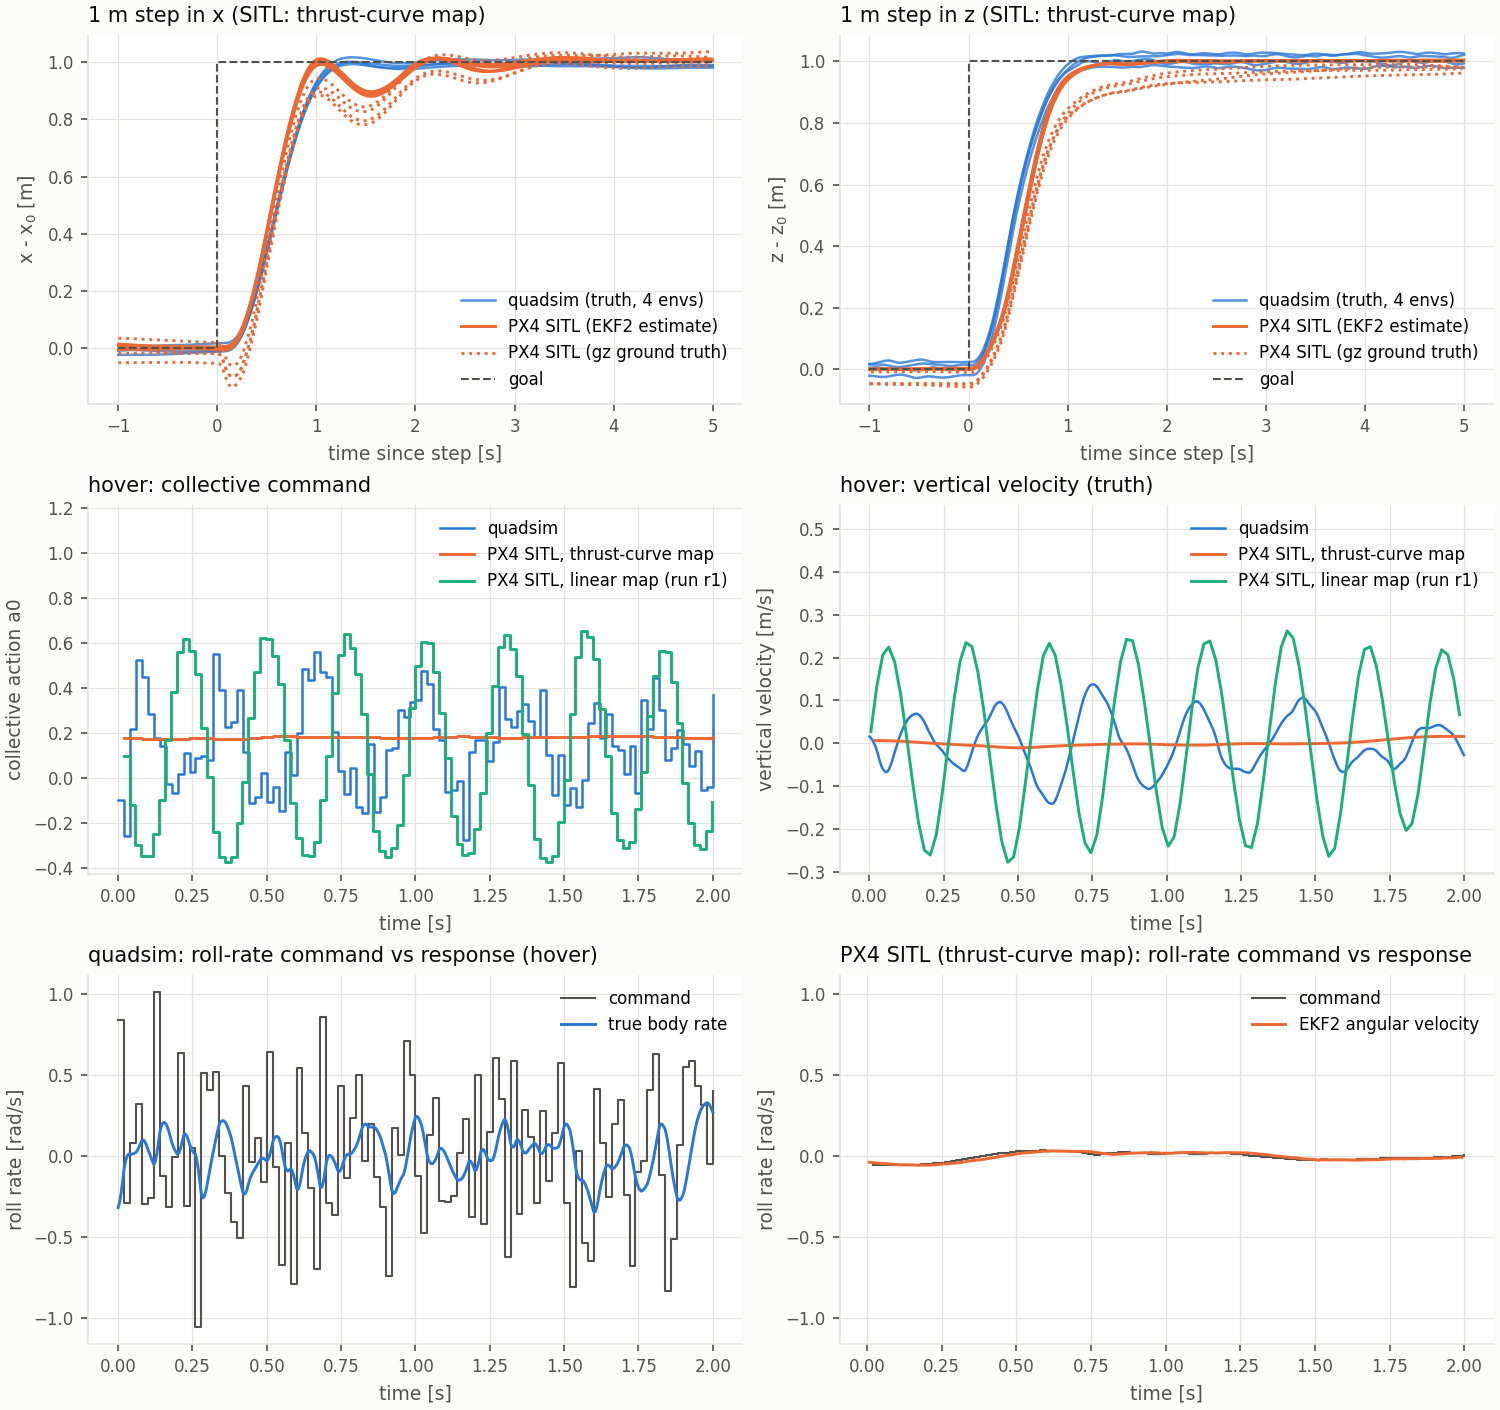
\includegraphics[width=\linewidth]{sitl_vs_quadsim.png}
\caption{Top: \SI{1}{m} steps (quadsim truth, SITL estimate and truth). Middle: hover collective command and vertical
velocity -- with the linear thrust map PX4 SITL shows a \SI{4}{Hz} heave limit cycle that the thrust-curve map removes.
Bottom: roll-rate command and response (quadsim commands chatter because of the white odometry noise).}
\label{fig:sitl-steps}
\end{figure}
Findings:
(i) \emph{Control performance transfers}: referenced to the estimate, SITL holds the pose to \SIrange{0.8}{1.0}{cm} RMS
(quadsim \SI{1.9}{cm}) and the $z$ step rises and settles as in quadsim; the smoother EKF2 estimate produces much quieter
commands than quadsim's white-noise odometry. (ii) The $x$ step settles slower in SITL (\SI{1.86}{s} vs \SI{1.07}{s}; the
position dips back to $\approx$\SI{0.9}{m}); the cause is not isolated (the pitch loop is not slower, see (iv)). (iii) \emph{Heave limit cycle}: with the
linear thrust map, 3 of 5 runs developed a persistent \SIrange{3.75}{4}{Hz} vertical oscillation (collective std 0.30--0.36,
vertical velocity 0.14--0.17\,m/s RMS) from the hand-over on; with the curve map 0 of 4 runs did. Quadsim shows the same
lightly damped mode as noise-driven heave; the 1.6$\times$ local thrust gain of the linear map turns it into a limit
cycle. (iv) \emph{Rate loop}: PX4's pitch response matches quadsim's delay (8--14 vs 13\,ms) with a smaller time constant
(38--44 vs 53\,ms); roll is slower (22--32\,ms) because the x500 airframe's allocation geometry
(\texttt{CA\_ROTOR*}=0.13/0.20--0.22\,m) differs from the gz rotor positions ($\pm$0.174\,m); setting the true geometry
reduced the roll delay by 4--12\,ms under matched conditions (2 runs). Fitted delays depend on the excitation by
$\pm$\SI{10}{ms} (closed-loop identification); with PX4's backward-differenced ground-truth rates all SITL delays appear
$\approx$\SI{10}{ms} longer. (v) PX4's hover-thrust estimate is 0.7295
(default \texttt{MPC\_THR\_HOVER} 0.60); without calibration ($s=1$, $-19\,\%$ thrust) the policy still flies but holds
\SI{1.3}{cm} low. (vi) Odometry is 5--16\,ms old at the policy step (median per run, max \SI{23}{ms}) -- at and above the
trained 0--10\,ms.

\subsection{Training distribution v1 and multi-seed comparison}\label{sec:v1}
The findings above define the v1 distribution (\cref{sec:dr}). Hover policies were trained with three seeds on v1 and
compared with three seeds of v0 (seed 42 plus two new seeds) in quadsim and in SITL (\cref{tab:hover-v1}).
\begin{table}[h]\centering\small
\resizebox{\linewidth}{!}{\begin{tabular}{lccc}\toprule
Metric & v0 (3 seeds) & v1 (3 seeds) & v2 (3 seeds)\\\midrule
quadsim, v0 distribution: success [\%] & 99.9 $\pm$ 0.0 & 99.7 $\pm$ 0.4 & 99.0 $\pm$ 0.6\\
quadsim, v0 distribution: final pos. error [cm] & 1.28 $\pm$ 0.07 & 1.83 $\pm$ 0.30 & 1.58 $\pm$ 0.12\\
quadsim, v1 distribution: success [\%] & 73.9 $\pm$ 2.0 & 74.4 $\pm$ 3.1 & 69.3 $\pm$ 5.7\\
quadsim, v1 distribution: final pos. error [cm] & 6.58 $\pm$ 0.12 & 6.77 $\pm$ 0.23 & 6.84 $\pm$ 0.14\\
quadsim, harsh OOD: success [\%] & 77.8 $\pm$ 1.2 & 66.0 $\pm$ 4.2 & 70.2 $\pm$ 2.0\\
quadsim, harsh OOD: crash [\%] & 3.7 $\pm$ 0.2 & 3.6 $\pm$ 0.4 & 3.4 $\pm$ 0.4\\
scenario $g=1.0$: hover RMS w.r.t. estimate [cm] & 1.87 $\pm$ 0.00 & 2.46 $\pm$ 0.32 & 1.95 $\pm$ 0.05\\
scenario $g=1.0$: collective std & 0.149 $\pm$ 0.016 & 0.211 $\pm$ 0.049 & 0.079 $\pm$ 0.003\\
scenario $g=1.6$: collective std & 0.209 $\pm$ 0.026 & 0.286 $\pm$ 0.079 & 0.112 $\pm$ 0.007\\
scenario $g=1.6$: vertical velocity RMS [cm/s] & 8.7 $\pm$ 1.0 & 9.0 $\pm$ 2.3 & 8.6 $\pm$ 0.8\\
SITL linear map: runs with limit cycle & 1 / 6 & 4 / 6 & 0 / 6\\
SITL curve map: runs with limit cycle & -- & 1 / 3 & 0 / 3\\
SITL linear map: collective std & 0.061 $\pm$ 0.080 & 0.310 $\pm$ 0.171 & 0.062 $\pm$ 0.016\\
SITL linear map: hover RMS w.r.t. estimate [cm] & 1.00 $\pm$ 0.10 & 2.17 $\pm$ 0.27 & 1.26 $\pm$ 0.23\\
SITL linear map: $x$ step settling [s] & 1.02 $\pm$ 0.02 & 1.05 $\pm$ 0.01 & 0.99 $\pm$ 0.05\\
SITL curve map: collective std & -- & 0.164 $\pm$ 0.142 & 0.031 $\pm$ 0.025\\
SITL curve map: hover RMS w.r.t. estimate [cm] & -- & 2.16 $\pm$ 0.74 & 1.29 $\pm$ 0.21\\
\bottomrule\end{tabular}
}
\caption{Hover policies trained on v0 vs v1, mean $\pm$ std over 3 seeds. Quadsim: 1000 episodes per seed and
condition; scenario: hover + steps with nominal dynamics and a thrust-map gain $g$ (1.6 = linear map on the gz x500).
SITL: limit-cycle runs = collective std $>0.1$ in hover. Source: \texttt{docs/results/hover\_v1.json}.}
\label{tab:hover-v1}
\end{table}
\TBD{v1 findings}

\subsection{Trajectory tracking and waypoints}
\Cref{tab:sitl-tasks} compares the tracking policy on a circle ($r=\SI{1}{m}$, \SI{0.2}{Hz}, \SI{1.26}{m/s}) and a figure-8
($r=\SI{1.5}{m}$, \SI{0.15}{Hz}) and the waypoint policy on a fixed 5-waypoint course, all with the thrust-curve map.
Referenced to the estimate, tracking in SITL equals quadsim (circle 2.2 vs \SI{2.5}{cm}, figure-8 3.4 vs \SI{3.0}{cm} RMSE);
the truth-referenced error is 3--4$\times$ larger because of EKF2's correlated error. The waypoint course was completed
in every SITL run (policy's own estimate-based switching) but took \SI{6.7}{s} instead of \SI{5.1}{s}; at up to
\SI{7}{m/s} EKF2's error reaches \SI{30}{cm}, so on truth some waypoints were passed just outside the \SI{0.3}{m} radius.
Removing quadsim's body drag did not change its time (\SI{5.13}{s}) and fixing the allocation geometry did not change
SITL's; PX4's saturation handling and slower inner loop are the remaining, not isolated, candidates.
\begin{table}[h]\centering\small
\begin{tabular}{llcc}\toprule
Task & Metric & quadsim & PX4 SITL\\\midrule
Tracking, circle (r 1 m, 0.2 Hz) & RMSE truth [cm] & 1.8 $\pm$ 0.4 & 6.3 $\pm$ 0.7\\
 & RMSE w.r.t. estimate [cm] & 2.5 $\pm$ 0.1 & 2.2 $\pm$ 0.2\\
Tracking, figure-8 (r 1.5 m, 0.15 Hz) & RMSE truth [cm] & 2.7 $\pm$ 0.2 & 9.2 $\pm$ 0.4\\
 & RMSE w.r.t. estimate [cm] & 3.0 $\pm$ 0.1 & 3.4 $\pm$ 0.4\\
Waypoints (5) & course completed & 1.00 & 1.00\\
 & time to finish [s] & 5.13 $\pm$ 0.02 & 6.74 $\pm$ 0.27\\
 & estimate error during course, RMS [cm] & -- & 15.2 $\pm$ 0.7\\
\bottomrule\end{tabular}

\caption{Tracking and waypoint policies (v0), quadsim (32 envs) vs PX4 SITL (2 runs each); RMSE after the first
\SI{2}{s}. Source: \texttt{docs/results/sitl\_tasks.json}.}
\label{tab:sitl-tasks}
\end{table}

\subsection{Obstacle navigation through the velocity interface}
The range-ring navigation policy commands velocities, which PX4's position controller tracks. Obstacles are virtual in
SITL: a 2-D LiDAR node ray-casts the training ring against the cylinders of a layout from the ground-truth pose (identical
to the training caster, unit-tested), and collisions are evaluated from the ground truth with the training criterion. Six
layouts drawn from the full-density training distribution were flown once in SITL and by 32 quadsim environments each
(\cref{tab:sitl-nav}). With PX4's default velocity controller only 2 of 6 SITL flights reached the goal, against 87\,\%
quadsim success on the same layouts. Identifying both velocity loops from the flight data explains the gap: PX4's
lateral velocity response has $L=\SI{0.22}{s}$, $\tau=\SI{0.44}{s}$ (VAF 0.85) against $L=\SI{0.14}{s}$, $\tau=\SI{0.22}{s}$
for quadsim's simulated cascade -- PX4's default horizontal velocity gain (\texttt{MPC\_XY\_VEL\_P\_ACC}=1.8) is lower than the
simulated one (3.0), so avoidance manoeuvres arrive late. Configuring PX4's velocity controller like the training cascade
(\texttt{MPC\_XY\_VEL\_P\_ACC}=3.0, D=0, \texttt{MPC\_Z\_VEL\_I\_ACC}=1.0, tilt limit 0.6\,rad) reduced the lateral time constant
to \SI{0.25}{s} (quadsim \SI{0.22}{s}) and doubled the SITL success to 4 of 6 layouts; the remaining failures are layout~1
(hard in quadsim as well, 38\,\% success) and layout~4. The residual lateral delay ($\approx$\SI{0.21}{s} vs \SI{0.14}{s})
comes from PX4's attitude and rate chain and is not represented in training. With one SITL flight per layout these rates
are indicative only; the lesson for deployment is that velocity-interface policies must be trained with the target
autopilot's velocity-loop dynamics (identified, or randomized over a range that contains them).
\begin{table}[h]\centering\small
\resizebox{\linewidth}{!}{\begin{tabular}{ccccc}\toprule
Layout & obstacles & quadsim success / collision [\%] & PX4 default velocity loop & PX4 velocity loop matched to quadsim\\\midrule
0 & 7 & 100 / 0 & goal & goal\\
1 & 15 & 38 / 62 & collision & collision\\
2 & 13 & 97 / 3 & goal & goal\\
3 & 15 & 97 / 3 & collision & goal\\
4 & 11 & 91 / 6 & collision & collision\\
5 & 15 & 100 / 0 & collision & goal\\
\bottomrule\end{tabular}
}
\caption{Navigation layouts: quadsim success / collision rate (32 envs per layout) and the outcome of the PX4 SITL flight
with PX4's default and with a quadsim-matched velocity controller. Source: \texttt{docs/results/sitl\_tasks.json}.}
\label{tab:sitl-nav}
\end{table}

\subsection{Summary of the cross-check}
\begin{itemize}
\item All CTBR policies (hover, tracking, waypoints) fly PX4 SITL as offboard controllers; at the level the policy
controls (estimate-referenced) their performance matches quadsim; the bridge's safety gating is verified.
\item Sim-to-sim gaps were found and quantified, each with an identified cause: EKF2's correlated error (training model too
white), GNSS delay mis-configuration in SITL, the thrust-map nonlinearity (heave limit cycle; fixed by the curve map),
PX4's roll/pitch-asymmetric rate loop (allocation geometry), up to \SI{20}{ms} observation age, and -- the
largest -- PX4's slower velocity loop for the velocity-interface navigation policy.
\item Not done: hardware flights, depth/RGB policies in SITL (needs a rendered camera in gz), retraining the
navigation policy with a randomized velocity loop.
\end{itemize}


%==========================================================================================
\section{From platform to research framework}\label{sec:framework}
The platform of the previous sections was built around a fixed set of tasks. An audit of that code base for
reuse by other researchers found four structural limits: (i) the action interfaces were branches of one controller
function, so a new interface required editing the base environment; (ii) vehicles were two hard-coded Python presets
(quadrotors only for direct motor control); (iii) observations, rewards, terminations and randomizations could only be
extended by subclassing a task; (iv) training was tied to one algorithm library, with a separate, non-competitive SAC
script, and there were no standard benchmark conditions, no constrained or multi-agent tasks and no
imitation-learning data path. This section describes the framework that replaced these limits without rebuilding the
validated core, and the experiments that validate it. Architecture details are in \texttt{docs/FRAMEWORK.md}.

\subsection{Extension points}
Every replaceable component type has a name registry; components register themselves on import, research code
registers its own (from any module or file passed as \texttt{--plugins} to every script) and selects them by name in
the configuration or on the command line (\cref{tab:ext}). Configuration-level extensions do not need a registry:
each task configuration carries \emph{terms} with the Isaac~Lab signature \texttt{func(env, **params)}
(\cref{tab:terms}).

\begin{table}[!htbp]\centering\small
\caption{Registries (\texttt{quadsim.registry}).}\label{tab:ext}
\begin{tabularx}{\linewidth}{lXX}\toprule
Registry & Selected by & Built-in components\\\midrule
\texttt{VEHICLES} & \texttt{dynamics.preset} (name or YAML/JSON file) & x500, crazyflie, racer5, hexa\_x\\
\texttt{ACTION\_INTERFACES} & \texttt{control.mode} & motor, ctbr, ctatt, velocity, position\\
\texttt{ALGORITHMS} & \texttt{--algo} & ppo (rsl\_rl), sac, td3, bc, vla\\
\texttt{BASELINES} & \texttt{--controllers} & cascade, geometric, potential\_field, swarm\_potential, langnav\_expert\\
\texttt{BENCHMARKS} & \texttt{benchmark/run.py --suite} & hover, track, waypoint, nav\_range, race, swarm, langnav\\
\bottomrule\end{tabularx}
\end{table}

\begin{table}[!htbp]\centering\small
\caption{Configurable MDP terms (\texttt{cfg.terms}).}\label{tab:terms}
\begin{tabularx}{\linewidth}{lX}\toprule
Term & Semantics\\\midrule
observation & appended to the deployable policy observation (or the critic's, if privileged) with sampling period
$P$, latency $D$, white noise, scale, clip and an optional history of $H$ samples\\
reward & $w\,f(s_t)\,\Delta t$, logged per term\\
termination & failure, or truncation (bootstrapped)\\
cost & constraint cost rate $c(s_t)\ge0$; episode cost $J_c=\sum_t c\,\Delta t$ (seconds of violation for an indicator)\\
event & start-up / reset / interval randomization or perturbation\\
curriculum & called before resets with the finished episodes' metrics (e.g.\ raise the initial tilt when success $>80\,\%$)\\
\bottomrule\end{tabularx}
\end{table}

\paragraph{Sensor terms.} A term $h$ with period $P$ and latency $D$ (both in policy steps) produces
$o_t=h\big(s_{P\lfloor (t-D)/P\rfloor}\big)+\eta$, $\eta\sim\mathcal N(0,\sigma^2 I)$, with the history refilled at
every episode start. The same mechanism implements a 5\,Hz GNSS fix with \SI{100}{ms} latency, a downward rangefinder,
a 3-D LiDAR ray-casting the task's obstacle primitives, or action/gyro histories for implicit adaptation.

\paragraph{Vehicles.} A vehicle file may inherit from a preset, generate a symmetric $n$-rotor frame (4-rotor X frames
use the PX4 Quad-X numbering), derive $k_f$ from the thrust-to-weight ratio and estimate the inertia from a box body
and point-mass motors. Vehicles are rejected if the inertia violates the triangle inequality, the thrust-to-weight
ratio is $\le1.05$ or the allocation matrix $A\in\R^{4\times n}$ (collective, roll, pitch, yaw) has rank $<4$. The
USD body, PhysX mass properties, motor and drag model, pseudo-inverse mixer with PX4-style desaturation, hover action
and the motor-level action dimension follow automatically. An Isaac~Lab \texttt{MultirotorCfg} (allocation matrix with
rows $[F_x,F_y,F_z,M_x,M_y,M_z]$, thrust $c\,\mathrm{rps}^2$) converts with $y_i=A_{3i}$, $x_i=-A_{4i}$,
$s_i=-\mathrm{sign}A_{5i}$, $k_f=c/(2\pi)^2$.

\paragraph{Constrained RL.} With cost terms and \texttt{safety.lagrangian}, the environment optimizes the Lagrangian
of $\max_\pi J_r(\pi)$ s.t.\ $J_c(\pi)\le d$ by returning $\tilde r_t=(r_t-\lambda c_t)/(1+\lambda)$ to \emph{any} RL
algorithm and updating $\lambda$ with the PID rule of Stooke et al.~\cite{stooke2020pid}: $e_k=\bar J_c-d$,
$I_k=\max(0,I_{k-1}+K_ie_k)$, $\lambda_k=\min\!\big(\lambda_{\max},\max(0,K_pe_k+I_k+K_d\max(0,\bar J_{c,k}-\bar J_{c,k-1}))\big)$,
where $\bar J_c$ is the mean cost of the episodes finished since the last update (every rollout). This is the
reward-penalty form (no separate cost critic).

\paragraph{Multi-agent RL.} $M$ consecutive environment rows form a team sharing a local frame, an episode clock and
resets; each agent is one row. Any single-agent algorithm therefore trains a parameter-shared decentralized policy
$\pi(a^i\mid o^i)$, while the critic receives the centralized state (true relative states and goals of all team
members), i.e.\ a MAPPO-style~\cite{yu2022mappo} centralized-training, decentralized-execution scheme. A crash terminates the crashed
agent and truncates its teammates; inter-agent collisions are analytic.

\paragraph{Off-policy learning.} The original skrl SAC~\cite{haarnoja2018sac} reached 0\,\% hover success. Two likely causes were addressed
together (not ablated separately): the tasks' rewards are $\Delta t$-scaled (about $0.02$ per step), so the entropy
bonus dominated, and the critic only saw the policy observation; the update-to-data ratio was also low (1/256). The framework's SAC/TD3 use asymmetric twin critics with LayerNorm on the
privileged observation, running observation normalization, rewards in per-second units ($r/\Delta t$), 1024 parallel
environments, batches of 16\,384 and 4 gradient updates per environment step, following the many-environment recipe of FastTD3~\cite{seo2025fasttd3}; TD3~\cite{fujimoto2018td3} shares the implementation. Time-outs bootstrap from the current
state (as in rsl\_rl's PPO).

\paragraph{Imitation learning and VLA.} Demonstrations are episode-structured HDF5 files (policy and critic
observations, camera frames, actions, rewards, ground truth, estimate, instruction text, success, metrics,
configuration, observation layout, tokenizer). Collection gives every environment the same episode quota, because
stopping at a global count discards the episodes still running, which are the long ones. Behaviour cloning minimizes
$\mathbb E\|\pi_\theta(o)-a^\star\|^2$; instruction tokens are embedded with a bag-of-words encoder that ignores
padding and out-of-vocabulary words, and images are encoded by a CNN whose last feature map is FiLM-modulated~\cite{perez2018film} by the
instruction embedding. DAgger~\cite{ross2011dagger} alternates rollouts of the learner (labelled by the expert) with retraining on the
aggregated data. External VLA models plug in through an adapter $(\text{images},\text{instructions},
\text{proprioception})\mapsto a$; datasets export to the LeRobot~\cite{cadene2024lerobot} v3.0 format and are verified by reloading them with
LeRobot's own loader.

\paragraph{Benchmarks.} A suite fixes a task, a set of conditions labelled in-distribution (training distribution)
or out-of-distribution (wind and pushes, harsh dynamics, sensor noise $\times2$--3, \SIrange{20}{30}{ms} command plus
\SIrange{0}{30}{ms} estimate latency,
unseen layouts or phrasings), metrics and seeds. Every controller is evaluated per condition in a fresh simulator
process with the same seed; the report gives each metric with its 95\,\% CI and the generalization gap
$\text{id}-\overline{\text{ood}}$ of the primary metric.

\paragraph{Resources.} The default number of environments is lowered automatically when the free GPU memory would
not fit it (memory model calibrated on the RTX~5060 measurements; never raised unless requested).

\subsection{Validation of the framework}
\paragraph{Regression.} After moving the action interfaces into classes, the vehicles into a registry and adding the
term machinery, the reference evaluations (hover, tracking, waypoint, range navigation; PPO policies and the cascade,
SE(3) and potential-field baselines) were re-run: all 59 metrics are bit-identical to the pre-refactor run, both
after the refactor and with the final code.
\paragraph{Unit and example tests.} 124 CPU unit tests at the framework milestone (141 after the review) (registries, vehicle files and frames, allocation rank, Isaac Lab
conversion, hover action of every interface on every vehicle, closed-loop position control of a hexarotor and a
racer on the reference integrator, sensor-term rate/latency/history, the PID multiplier, the squashed-Gaussian
log-likelihood, replay buffer, hardware model, tokenizer, datasets, BC language grounding) and an example check that
runs every extension example in the simulator (\cref{tab:fw_examples}).

\begin{figure}[!htbp]\centering
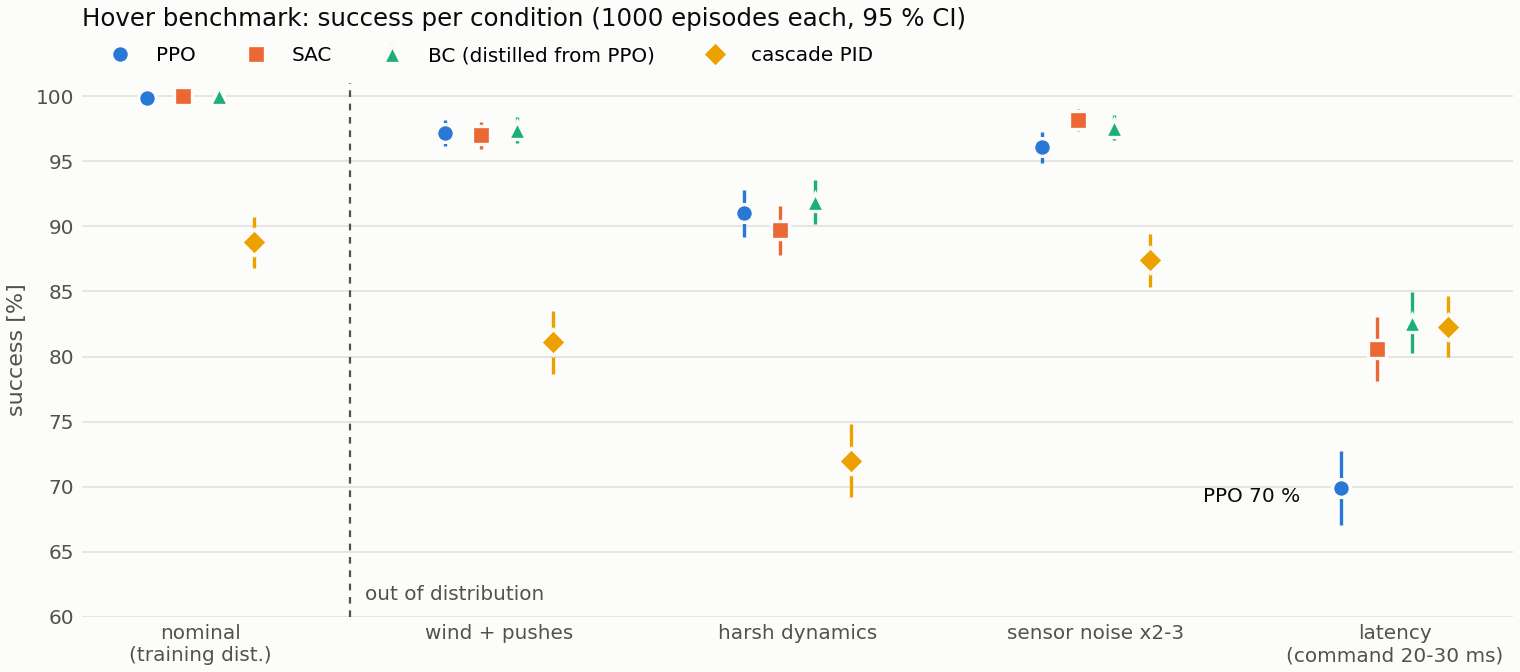
\includegraphics[width=\linewidth]{framework_hover_benchmark.png}
\caption{Hover benchmark suite: success per evaluation condition for PPO, the framework's SAC, a BC student distilled
from the PPO policy and the cascade baseline (1000 episodes per point, same seed, 95\,\% CI; values in
\cref{tab:fw_algos}).}\label{fig:fw_bench}
\end{figure}

\begin{table}[!htbp]\centering\small\caption{Hover benchmark suite: success per condition (1000 episodes each, same seed, fresh process per controller and condition) and generalization gap id$-$mean(ood) in points. Source: \texttt{docs/results/framework/bench\_hover\_algos.json}.}\label{tab:fw_algos}
\begin{adjustbox}{max width=\linewidth}\begin{tabular}{lcccccc}\toprule
Controller & nominal (id) & wind\_push & harsh\_dynamics & sensor\_noise & latency & gap\\\midrule
ppo & 99.9\,\% & 97.2\,\% & 91.0\,\% & 96.1\,\% & 69.9\,\% & +11.4\\
sac & 100.0\,\% & 97.0\,\% & 89.7\,\% & 98.2\,\% & 80.6\,\% & +8.6\\
bc\_distilled & 100.0\,\% & 97.4\,\% & 91.9\,\% & 97.6\,\% & 82.6\,\% & +7.6\\
cascade & 88.8\,\% & 81.1\,\% & 72.0\,\% & 87.4\,\% & 82.3\,\% & +8.1\\
\bottomrule\end{tabular}\end{adjustbox}
\end{table}

\begin{table}[!htbp]\centering\small\caption{Learning algorithms on hover (nominal condition, 1000 episodes). Position error in cm, yaw error in rad. Source: \texttt{offpolicy\_hover.json}.}\label{tab:fw_offpolicy}
\begin{adjustbox}{max width=\linewidth}\begin{tabular}{lcccc}\toprule
Algorithm & Success & Pos. err [cm] & Yaw err [rad] & Train [min]\\\midrule
PPO (rsl\_rl), 4096 envs, 600 it. & 99.9\,\% & 1.26\,$\pm$\,0.04 & 0.08\,$\pm$\,0.00 & --\\
SAC (quadsim), 1024 envs, 15k steps & 100.0\,\% & 1.67\,$\pm$\,0.05 & 0.51\,$\pm$\,0.01 & 21\\
TD3 (quadsim), 1024 envs, 15k steps & 0.0\,\% & 87.49\,$\pm$\,1.77 & 0.63\,$\pm$\,0.02 & 19\\
TD3, noise 0.05-0.15, reward scale 10, 8 upd./step & 99.9\,\% & 2.73\,$\pm$\,0.24 & 1.06\,$\pm$\,0.01 & 28\\
ARS (plugin example), 150 it. & 46.8\,\% & 11.87\,$\pm$\,0.40 & 0.58\,$\pm$\,0.04 & 12\\
\bottomrule\end{tabular}\end{adjustbox}
\end{table}

\begin{table}[!htbp]\centering\small\caption{New vehicles, control interfaces and tasks defined through the extension points (1000 episodes; position error in cm). Source: \texttt{vehicles\_interfaces.json}.}\label{tab:fw_vehicles}
\begin{adjustbox}{max width=\linewidth}\begin{tabular}{lccc}\toprule
Configuration & Success & Pos. err [cm] & Crash\\\midrule
hexa\_x (6 rotors, generated frame), CTBR, PPO & 99.8\,\% & 1.21\,$\pm$\,0.03 & 0.0\,\%\\
hexa\_x, cascade baseline & 96.2\,\% & 4.46\,$\pm$\,0.68 & 0.3\,\%\\
hexa\_x, motor-level (6-D action), PPO & 100.0\,\% & 1.40\,$\pm$\,0.04 & 0.0\,\%\\
x500, acceleration interface (plugin example), PPO & 99.7\,\% & 1.40\,$\pm$\,0.05 & 0.0\,\%\\
landing task (plugin example), PPO, first reward & 0.0\,\% & -- & 0.5\,\%\\
landing task, PPO, reward v2 (time penalty, low-and-slow term) & 94.1\,\% & -- & 5.9\,\%\\
landing task, cascade baseline & 64.1\,\% & -- & 35.9\,\%\\
\bottomrule\end{tabular}\end{adjustbox}
\end{table}

\begin{table}[!htbp]\centering\small\caption{Constrained waypoint racing: speed $\le$\,\SI{2}{m/s}, budget \SI{0.1}{s} of over-speed flight per episode (500 episodes). Source: \texttt{safe\_rl.json}.}\label{tab:fw_safe}
\begin{adjustbox}{max width=\linewidth}\begin{tabular}{lcccc}\toprule
Policy & Success & Episode cost [s] & Time [s] & Crash\\\midrule
PPO (unconstrained) & 99.4\,\% & 5.350\,$\pm$\,0.076 & 6.66\,$\pm$\,0.11 & 0.6\,\%\\
cascade & 91.6\,\% & 6.503\,$\pm$\,0.123 & 10.38\,$\pm$\,0.15 & 2.0\,\%\\
PPO-Lagrangian (PID multiplier) & 87.6\,\% & 0.081\,$\pm$\,0.017 & 11.89\,$\pm$\,0.15 & 0.0\,\%\\
\bottomrule\end{tabular}\end{adjustbox}
\end{table}

\begin{table}[!htbp]\centering\small\caption{Drone racing (2 laps, 7 gates, 5-inch racer); trained on random circuits. Source: \texttt{bench\_race.json}.}\label{tab:fw_race}
\begin{adjustbox}{max width=\linewidth}\begin{tabular}{llcccc}\toprule
Controller & Condition & success & lap\_time & gates\_passed & crash\\\midrule
cascade & random\_tracks (id) & 0.6\,\% & 15.04\,$\pm$\,0.32 & 6.62\,$\pm$\,0.28 & 25.2\,\%\\
cascade & ellipse (ood) & 0.0\,\% & 15.22\,$\pm$\,0.31 & 7.14\,$\pm$\,0.26 & 14.4\,\%\\
cascade & figure8 (ood) & 0.0\,\% & 18.42\,$\pm$\,0.18 & 6.06\,$\pm$\,0.21 & 16.0\,\%\\
cascade & wind (ood) & 0.6\,\% & 15.08\,$\pm$\,0.32 & 6.28\,$\pm$\,0.29 & 27.8\,\%\\
ppo & random\_tracks (id) & 94.4\,\% & 2.47\,$\pm$\,0.02 & 13.49\,$\pm$\,0.20 & 5.6\,\%\\
ppo & ellipse (ood) & 99.6\,\% & 2.49\,$\pm$\,0.01 & 13.96\,$\pm$\,0.06 & 0.4\,\%\\
ppo & figure8 (ood) & 5.4\,\% & 4.15\,$\pm$\,0.05 & 3.40\,$\pm$\,0.39 & 94.6\,\%\\
ppo & wind (ood) & 95.8\,\% & 2.47\,$\pm$\,0.02 & 13.63\,$\pm$\,0.17 & 4.2\,\%\\
ppo\_v1 & random\_tracks (id) & 94.8\,\% & 2.45\,$\pm$\,0.02 & 13.46\,$\pm$\,0.21 & 5.2\,\%\\
ppo\_v1 & ellipse (ood) & 98.0\,\% & 2.49\,$\pm$\,0.01 & 13.84\,$\pm$\,0.10 & 2.0\,\%\\
ppo\_v1 & figure8 (ood) & 73.8\,\% & 3.73\,$\pm$\,0.02 & 12.90\,$\pm$\,0.50 & 26.2\,\%\\
ppo\_v1 & wind (ood) & 95.4\,\% & 2.47\,$\pm$\,0.02 & 13.56\,$\pm$\,0.19 & 4.6\,\%\\
\bottomrule\end{tabular}\end{adjustbox}
\end{table}

\begin{table}[!htbp]\centering\small\caption{Four-agent antipodal swap (shared policy, centralized critic). Source: \texttt{bench\_swarm.json}.}\label{tab:fw_swarm}
\begin{adjustbox}{max width=\linewidth}\begin{tabular}{llcccc}\toprule
Controller & Condition & success & agent\_collision & min\_separation & time\_to\_goal\\\midrule
cascade & swap4 (id) & 35.9\,\% & 36.1\,\% & 0.95\,$\pm$\,0.02 & 2.28\,$\pm$\,0.03\\
cascade & wind (ood) & 29.7\,\% & 36.9\,\% & 0.95\,$\pm$\,0.02 & 2.30\,$\pm$\,0.03\\
cascade & latency (ood) & 35.9\,\% & 33.8\,\% & 0.95\,$\pm$\,0.02 & 2.24\,$\pm$\,0.02\\
ppo & swap4 (id) & 87.5\,\% & 0.4\,\% & 1.39\,$\pm$\,0.02 & 2.04\,$\pm$\,0.04\\
ppo & wind (ood) & 89.8\,\% & 0.8\,\% & 1.37\,$\pm$\,0.02 & 2.09\,$\pm$\,0.06\\
ppo & latency (ood) & 80.5\,\% & 1.2\,\% & 1.38\,$\pm$\,0.02 & 2.16\,$\pm$\,0.07\\
swarm\_potential & swap4 (id) & 100.0\,\% & 0.0\,\% & 1.28\,$\pm$\,0.01 & 6.89\,$\pm$\,0.08\\
swarm\_potential & wind (ood) & 97.7\,\% & 0.0\,\% & 1.29\,$\pm$\,0.01 & 6.80\,$\pm$\,0.07\\
swarm\_potential & latency (ood) & 96.1\,\% & 0.0\,\% & 1.24\,$\pm$\,0.01 & 6.94\,$\pm$\,0.08\\
\bottomrule\end{tabular}\end{adjustbox}
\end{table}

\begin{table}[!htbp]\centering\small\caption{Imitation learning. Hover: RL-to-BC distillation (last column: final position error [cm]). LangNav: success with training / held-out instruction phrasings and wrong-landmark rate (training phrasing). Source: \texttt{imitation.json}.}\label{tab:fw_il}
\begin{adjustbox}{max width=\linewidth}\begin{tabular}{llccc}\toprule
Task & Policy & Success (train phr.) & Success (held-out) & Wrong / pos. err\\\midrule
hover & PPO teacher & 99.9\,\% & -- & 1.26\,$\pm$\,0.04\\
hover & BC student & 99.9\,\% & -- & 1.26\,$\pm$\,0.04\\
hover & BC student, no last action & 100.0\,\% & -- & 1.32\,$\pm$\,0.04\\
langnav (map) & scripted expert (privileged) & -- & 100.0\,\% & --\\
langnav (map) & BC (with last action) & 15.4\,\% & 41.0\,\% & 0.2\,\%\\
langnav (map) & BC, instruction removed & 10.8\,\% & 10.8\,\% & 10.0\,\%\\
langnav (map) & BC, no last action, unknown words averaged in & 81.0\,\% & 30.8\,\% & 0.0\,\%\\
langnav (map) & same policy, unknown words ignored & 81.0\,\% & 58.2\,\% & 0.0\,\%\\
langnav (map) & + DAgger round 1 & 100.0\,\% & 50.8\,\% & 0.0\,\%\\
langnav (map) & + DAgger round 2 & 100.0\,\% & 56.2\,\% & 0.0\,\%\\
langnav (map) & same data, frozen CLIP text encoder & 100.0\,\% & 97.0\,\% & 0.0\,\%\\
langnav (RGB) & scripted expert (privileged) & 100.0\,\% & -- & 0.0\,\%\\
langnav (RGB) & BC, FiLM-CNN + instruction & 82.8\,\% & 85.3\,\% & 0.0\,\%\\
langnav (RGB) & + DAgger round 1 & 100.0\,\% & 100.0\,\% & 0.0\,\%\\
langnav (RGB) & same data, frozen CLIP text encoder & 99.7\,\% & 99.1\,\% & 0.0\,\%\\
langnav (RGB) & VLA adapter: colour servo & 6.6\,\% & 7.2\,\% & 0.0\,\%\\
langnav (RGB) & BC, demonstrations re-collected (camera fix) & 83.8\,\% & 90.9\,\% & 0.0\,\%\\
langnav (RGB) & + DAgger round 1, re-collected & 100.0\,\% & 100.0\,\% & 0.0\,\%\\
langnav (RGB) & SmolVLA fine-tuned, 10 actions per chunk & 19.1\,\% & 19.4\,\% & 50.3\,\%\\
langnav (RGB) & SmolVLA fine-tuned, 50 actions per chunk & 27.2\,\% & 22.2\,\% & 59.7\,\%\\
langnav (RGB) & SmolVLA fine-tuned, re-planned every step & -- & 12.2\,\% & --\\
langnav (RGB) & SmolVLA after 5k of the 10k steps, 10 per chunk & 12.8\,\% & -- & 31.9\,\%\\
langnav (RGB) & SmolVLA, empty instruction, 10 per chunk & 19.7\,\% & -- & 59.4\,\%\\
\bottomrule\end{tabular}\end{adjustbox}
\end{table}

\begin{table}[!htbp]\centering\small\caption{Multi-seed replication: the published single-seed runs (seed 42; BC seed 0) and two more seeds with identical configurations; mean $\pm$ sample std over seeds and a stratified bootstrap 95\,\% CI of the mean over seeds. BC seeds vary initialization and train/validation split on the same demonstrations. Source: \texttt{multiseed.json}.}\label{tab:fw_multiseed}
\begin{adjustbox}{max width=\linewidth}\begin{tabular}{lccccc}\toprule
Result & Seed 42 / 0 & Seed 1 & Seed 2 & Mean $\pm$ std & 95\,\% CI\\\midrule
Race-v0, success [\%], random tracks & 94.4 & 97.2 & 96.8 & 96.1\,$\pm$\,1.5 & [94.4, 97.2]\\
Race-v0, success [\%], ellipse & 99.6 & 99.2 & 98.2 & 99.0\,$\pm$\,0.7 & [98.2, 99.6]\\
Race-v0, success [\%], figure8 & 5.4 & 6.4 & 0.4 & 4.1\,$\pm$\,3.2 & [0.4, 6.4]\\
Race-v0, success [\%], wind & 95.8 & 95.8 & 96.6 & 96.1\,$\pm$\,0.5 & [95.8, 96.6]\\
Race-v1 (both directions), success [\%], random tracks & 94.8 & 96.8 & 95.6 & 95.7\,$\pm$\,1.0 & [94.8, 96.8]\\
Race-v1 (both directions), success [\%], ellipse & 98.0 & 97.2 & 97.2 & 97.5\,$\pm$\,0.5 & [97.2, 98.0]\\
Race-v1 (both directions), success [\%], figure8 & 73.8 & 66.6 & 79.2 & 73.2\,$\pm$\,6.3 & [66.6, 79.2]\\
Race-v1 (both directions), success [\%], wind & 95.4 & 95.4 & 95.8 & 95.5\,$\pm$\,0.2 & [95.4, 95.8]\\
Race-v1, finish terminal, success [\%], random tracks & 90.4 & 95.8 & 94.0 & 93.4\,$\pm$\,2.7 & [90.4, 95.8]\\
Race-v1, finish terminal, success [\%], ellipse & 93.6 & 98.2 & 96.4 & 96.1\,$\pm$\,2.3 & [93.6, 98.2]\\
Race-v1, finish terminal, success [\%], figure8 & 43.0 & 21.6 & 74.2 & 46.3\,$\pm$\,26.5 & [21.6, 74.2]\\
Race-v1, finish terminal, success [\%], wind & 90.6 & 95.6 & 93.0 & 93.1\,$\pm$\,2.5 & [90.6, 95.6]\\
Swarm, success [\%], swap4 & 87.5 & 89.1 & 92.2 & 89.6\,$\pm$\,2.4 & [87.5, 92.2]\\
Swarm, success [\%], wind & 89.8 & 77.3 & 89.1 & 85.4\,$\pm$\,7.0 & [77.3, 89.8]\\
Swarm, success [\%], latency & 80.5 & 76.6 & 72.7 & 76.6\,$\pm$\,3.9 & [72.7, 80.5]\\
Swarm, agent collisions [\%], swap4 & 0.4 & 4.3 & 0.4 & 1.7\,$\pm$\,2.3 & [0.4, 4.3]\\
PPO-Lagrangian, episode cost [s] (budget 0.1) & 0.081 & 0.126 & 0.108 & 0.105\,$\pm$\,0.023 & [0.081, 0.126]\\
PPO-Lagrangian, success [\%] & 87.6 & 0.0 & 85.2 & 57.6\,$\pm$\,49.9 & [0.0, 87.6]\\
LangNav map, BC, unknown words averaged, success [\%], train phr. & 81.0 & 68.8 & 78.0 & 75.9\,$\pm$\,6.4 & [68.8, 81.0]\\
LangNav map, BC, unknown words averaged, success [\%], held-out phr. & 30.8 & 15.6 & 14.4 & 20.3\,$\pm$\,9.1 & [14.4, 30.8]\\
LangNav map, BC, success [\%], train phr. & 81.0 & 68.8 & 78.0 & 75.9\,$\pm$\,6.4 & [68.8, 81.0]\\
LangNav map, BC, success [\%], held-out phr. & 58.2 & 64.0 & 62.4 & 61.5\,$\pm$\,3.0 & [58.2, 64.0]\\
LangNav map, DAgger-2, success [\%], train phr. & 100.0 & 100.0 & 100.0 & 100.0\,$\pm$\,0.0 & [100.0, 100.0]\\
LangNav map, DAgger-2, success [\%], held-out phr. & 56.2 & 84.2 & 80.0 & 73.5\,$\pm$\,15.1 & [56.2, 84.2]\\
LangNav map, DAgger-2 + CLIP, success [\%], train phr. & 100.0 & 100.0 & 100.0 & 100.0\,$\pm$\,0.0 & [100.0, 100.0]\\
LangNav map, DAgger-2 + CLIP, success [\%], held-out phr. & 97.0 & 95.6 & 98.0 & 96.9\,$\pm$\,1.2 & [95.6, 98.0]\\
LangNav RGB, BC, success [\%], train phr. & 82.8 & 75.3 & 71.9 & 76.7\,$\pm$\,5.6 & [71.9, 82.8]\\
LangNav RGB, BC, success [\%], held-out phr. & 85.3 & 75.3 & 62.8 & 74.5\,$\pm$\,11.3 & [62.8, 85.3]\\
LangNav RGB, DAgger-1, success [\%], train phr. & 100.0 & 100.0 & 100.0 & 100.0\,$\pm$\,0.0 & [100.0, 100.0]\\
LangNav RGB, DAgger-1, success [\%], held-out phr. & 100.0 & 95.3 & 100.0 & 98.4\,$\pm$\,2.7 & [95.3, 100.0]\\
LangNav RGB, DAgger-1 + CLIP, success [\%], train phr. & 99.7 & 100.0 & 99.7 & 99.8\,$\pm$\,0.2 & [99.7, 100.0]\\
LangNav RGB, DAgger-1 + CLIP, success [\%], held-out phr. & 99.1 & 99.7 & 100.0 & 99.6\,$\pm$\,0.5 & [99.1, 100.0]\\
LangNav RGB, re-collected data, BC, success [\%], train phr. & 83.8 & 83.8 & 73.1 & 80.2\,$\pm$\,6.1 & [73.1, 83.8]\\
LangNav RGB, re-collected data, BC, success [\%], held-out phr. & 90.9 & 82.8 & 59.1 & 77.6\,$\pm$\,16.6 & [59.1, 90.9]\\
LangNav RGB, re-collected data, DAgger-1, success [\%], train phr. & 100.0 & 100.0 & 99.4 & 99.8\,$\pm$\,0.4 & [99.4, 100.0]\\
LangNav RGB, re-collected data, DAgger-1, success [\%], held-out phr. & 100.0 & 100.0 & 97.5 & 99.2\,$\pm$\,1.4 & [97.5, 100.0]\\
\bottomrule\end{tabular}\end{adjustbox}
\end{table}

\begin{table}[!htbp]\centering\small\caption{Comparisons over seeds (Agarwal et al.~\cite{agarwal2021precipice}): probability that a random seed of X beats a random seed of Y on a random condition, and the interquartile mean of the success rate [\%], each with a stratified bootstrap 95\,\% CI. Source: \texttt{multiseed.json} (\texttt{comparisons}).}\label{tab:fw_compare}
\begin{adjustbox}{max width=\linewidth}\begin{tabular}{lccc}\toprule
Comparison X vs Y & P(X $>$ Y) & IQM X & IQM Y\\\midrule
Race v1 vs v0, figure-8 & 1.00 [1.00, 1.00] & 73.2 [66.6, 79.2] & 4.1 [0.4, 6.4]\\
Race v1 vs v0, all 4 conditions & 0.38 [0.25, 0.53] & 95.6 [95.2, 96.2] & 96.1 [95.2, 96.7]\\
Race v1, finish terminal vs time-out, all 4 conditions & 0.25 [0.06, 0.50] & 92.9 [91.4, 94.6] & 95.6 [95.2, 96.2]\\
LangNav map, CLIP vs bag of words (held-out phr.) & 1.00 [1.00, 1.00] & 96.9 [95.6, 98.0] & 73.5 [56.2, 84.2]\\
LangNav map, unknown words ignored vs averaged & 1.00 [1.00, 1.00] & 61.5 [58.2, 64.0] & 20.3 [14.4, 30.8]\\
LangNav RGB, DAgger-1 vs BC (both phrasings) & 1.00 [1.00, 1.00] & 100.0 [97.7, 100.0] & 76.3 [69.6, 82.2]\\
LangNav RGB BC, re-collected vs stale-frame data & 0.67 [0.33, 1.00] & 80.9 [69.6, 85.5] & 76.3 [69.6, 82.2]\\
LangNav RGB DAgger-1, re-collected vs stale-frame data & 0.44 [0.17, 0.67] & 99.8 [98.8, 100.0] & 100.0 [97.7, 100.0]\\
\bottomrule\end{tabular}\end{adjustbox}
\end{table}

\begin{table}[!htbp]\centering\small\caption{Extension examples executed in the simulator (\texttt{examples\_check.py}); success of the classical baseline where the check is an evaluation.}\label{tab:fw_examples}
\begin{adjustbox}{max width=\linewidth}\begin{tabular}{lcc}\toprule
Example & Result & Baseline success\\\midrule
vehicle\_yaml\_hexa & pass & 95\,\%\\
vehicle\_yaml\_inherit & pass & 52\,\%\\
vehicle\_plugin\_quad250 & pass & 61\,\%\\
sensor\_gnss & pass & --\\
task\_landing & pass & --\\
task\_landing\_baseline & pass & 58\,\%\\
reward\_curriculum & pass & --\\
action\_interface\_accel & pass & --\\
algorithm\_ars & pass & --\\
vla\_adapter\_color\_servo & pass & 7\,\%\\
sensor\_lidar\_nav & pass & 43\,\%\\
\bottomrule\end{tabular}\end{adjustbox}
\end{table}



\subsection{Findings}
All numbers below are the values re-measured after the review (\cref{sec:review}); racing, the swarm, the Lagrangian
and the language tasks are given over three seeds.
\begin{itemize}
\item \textbf{Algorithms (\cref{tab:fw_offpolicy,tab:fw_algos,fig:fw_bench}).} With the changes above SAC matches
PPO's in-distribution hover success ($\approx$100\,\%) in 21 instead of 8 minutes, with a slightly larger position error and a
much larger yaw error (its entropy term makes it indifferent to the weakly rewarded yaw). Out of distribution, PPO is
the most sensitive to latency beyond its training range (70\,\% vs 81--83\,\% for SAC and the BC student), so the
benchmark exposes a property that the in-distribution number hides. TD3 with the SAC configuration did not learn;
with smaller exploration noise, a smaller reward scale and 8 updates per step it reaches 99.9\,\%. A plug-in Augmented
Random Search (linear policy) reaches 46.8\,\% in 12 minutes.
\item \textbf{Generality (\cref{tab:fw_vehicles}).} A six-rotor vehicle generated from a frame description trains to
99.8\,\% with the unchanged task, and the extension examples (vehicle files, sensor terms, a new task, a new control
interface, a new algorithm) run through the unmodified scripts.
\item \textbf{Racing (\cref{tab:fw_race,tab:fw_multiseed}).} PPO completes two laps on $96\pm2$\,\% of unseen random
circuits at \SI{11.9}{m/s} mean speed (\SI{2.5}{s} per lap), transfers to a fixed reference circuit and to wind, but
rarely completes the figure-8 ($4\pm3$\,\%): the training circuits only turn counter-clockwise, the figure-8
alternates directions. Retraining with half of the circuits mirrored (both turning directions, same budget) raises the
figure-8 completion to $73\pm6$\,\% while keeping 95--98\,\% elsewhere --- the benchmark located the gap, a one-line
change of the training distribution closed most of it.
The classical cascade with gate-aligned waypoints passes about 7 of 14 gates in the episode (15\,s per lap, 25\,\%
crashes); its first version (straight to the gate centre) crashed into the frames in 99\,\% of the episodes.
\item \textbf{Multi-agent (\cref{tab:fw_swarm}).} The shared PPO policy coordinates four agents through the
antipodal swap (agent collisions 36\,\% for uncoordinated straight lines, $1.7\pm2.3$\,\% for PPO) and is 3.4 times
faster than a tuned potential field, which is, however, more reliable (100 vs $89.6\pm2.4$\,\% group success). The potential field's
gains were selected on the training scenario after its first setting failed (0\,\%, 53\,\% collisions).
\item \textbf{Constraints (\cref{tab:fw_safe,tab:fw_multiseed}).} The Lagrangian keeps the over-speed time around its
budget ($0.105\pm0.023$ vs \SI{0.1}{s} over three seeds) while the unconstrained policy spends \SI{5.4}{s} per course
above the limit; the price is a slower course and, in one of three seeds, a policy that never learned to finish the
course: its multiplier grew to $\approx$5 within 150 iterations, before the task was learned.
\item \textbf{Imitation and language (\cref{tab:fw_il}).} An RL policy distils into a BC student without loss. For
language-conditioned navigation, the last-action input makes BC copy its previous command and fail to stop (causal
confusion~\cite{dehaan2019causal}); removing it and two DAgger rounds reach the expert's 100\,\%. A bag-of-words
instruction encoder generalizes to unseen phrasings only if unknown words are ignored ($62\pm3$ vs $20\pm9$\,\% on the
same checkpoints) and then reaches $74\pm15$\,\% after DAgger, whereas a frozen pretrained CLIP text tower, with the
same data and policy, reaches $96.9\pm1.2$\,\%. With the RGB camera instead of the
landmark map (colours grounded in pixels), the FiLM-CNN policy reaches $77\pm6$\,\% and, after one DAgger round,
100\,\% (held-out phrasings $98\pm3$\,\%); its failures before DAgger were almost all collisions while approaching
(a wrong pillar in 1 of 320 episodes). A model-free colour-servo adapter exercises the VLA interface (7\,\%: correct
pillar, stopping rule outside the success zone).
\item \textbf{Defects found by the checks.} The example check found that observation terms were evaluated before
task buffers existed (now set up after the most-derived constructor) and that non-directory checkpoints (VLA
factories) were mistaken for run directories; a crashed simulator process hung for minutes holding GPU memory
(scripts now terminate after an exception). Demonstration collection stopping at a global episode count would bias
datasets toward short episodes (now a per-environment quota) --- the same stopping rule remained in the evaluator until
the review (\cref{sec:review}). The regression check was re-run after these fixes.
\end{itemize}

\subsection{Review, corrections and multi-seed replication}\label{sec:review}
\paragraph{Procedure.} After the framework milestone the code base was reviewed by three independent reviewers (one
for the core, vehicles, control interfaces and export; one for the task environments, terms and baselines; one for
the learning algorithms, imitation learning, evaluation and result tooling), each without access to the others'
findings, and the documentation was checked mechanically (every referenced file and task exists). Every reported
defect was reproduced before it was fixed --- on the CPU wherever possible, with a unit test that fails on the previous
code and passes after the fix (124 $\to$ 141 tests). The fixes were developed in a separate checkout while the
multi-seed training queue kept running on the unchanged code, so that all seeds of a task were trained with the same
code. \Cref{tab:review} lists the defects and their effect on published results.

\begin{table}[!htbp]\centering\small
\caption{Defects found by the review (effect on the results published before it, and the fix).}\label{tab:review}
\begin{tabularx}{\linewidth}{>{\raggedright\arraybackslash}X>{\raggedright\arraybackslash}p{0.27\linewidth}>{\raggedright\arraybackslash}p{0.2\linewidth}}\toprule
Defect & Effect on published results & Fix\\\midrule
Evaluator stopped at a global episode count and kept every finished episode: the episodes still running (the long
ones) were dropped & every evaluation; largest where outcomes differ in episode length & per-environment quota,
everything re-measured\\
Cascade baseline: velocity integrator not reset between episodes & cascade on hover, tracking, waypoints, racing &
reset per episode\\
Initial angular velocity written to PhysX in the world frame but used as a body rate by gyro, odometry and rate loop &
hover (first steps of an episode) & body-frame sample, rotated for PhysX\\
SAC Polyak-averaged its target critic twice per gradient step & published SAC run used $\tau_\text{eff}=0.00998$
(configuration said 0.005) & one update, default $\tau=0.01$\\
Off-policy resume acted randomly while refilling the replay buffer & none & policy refills the buffer\\
Curriculum averaged the last episode of every environment (mostly easier levels) and ran away & example only & judge
each level on its own episodes\\
Mixer used an equal collective split also for asymmetric layouts (torque at every thrust level) & none (presets
symmetric) & zero-torque split\\
\texttt{--plugins m.py env.a=b}: argparse attached the override to the plugin list & documented commands failed &
overrides recovered\\
Vehicle files: \texttt{1e-5} read as a string, invalid spins, \texttt{k\_f} together with thrust-to-weight, CoM
outside the rotor polygon accepted & none & typed parsing, validation\\
Hardware check counted the simulator's own memory twice & seed-42 safe-RL run used 3456 instead of 4096 environments &
own memory added back\\
Export: no plugins or overrides, exported network not taken from the algorithm, position contract incomplete & plug-in
tasks not exportable & completed\\
Result collector would have read the multi-seed tag as the curated race/swarm table; stale benchmark results reused
after a failure & latent & fixed sources, stale files removed\\
Rendered cameras: first frame of every episode showed the previous scene & RGB demonstrations ($\approx$0.7\,\% stale
frames) & re-render after resets\\
Race: 6.2\,\% of random circuits had overlapping gates, 0.22\,\% started inside a gate frame & random-circuit
conditions & resampled\\
LangNav: a dwell completed in a collision step counted as success and crash & 2 of 500 episodes & exclusive\\
Minor: unbounded cost list without Lagrangian, multiplier integral wind-up, silent reward-term override, ignored
\texttt{speed\_limit} override, BC on tiny datasets & none & fixed\\
\bottomrule\end{tabularx}
\end{table}

\paragraph{Evaluation sampling bias.} The evaluator ran $N$ parallel environments until the number of finished
episodes reached the requested $E$ and kept all of them. With $k=E/N\approx2$ episodes per environment this is a biased
sample: an environment whose episodes end early (a crash, an early success) contributes more of them, and the
episodes still running at the stopping time --- by the inspection paradox, preferentially the long ones --- are
discarded. Outcomes that end episodes early are therefore over-represented. In the extreme, the counter-clockwise
racing policy was reported at 0\,\% on the figure-8 because its few successful two-lap episodes ($\approx$\SI{7.4}{s})
had not finished when the crashed environments ($\approx$\SI{1}{s}) had produced the requested count. The corrected
evaluator takes the first $k=\lceil E/N\rceil$ episodes of every environment, which is unbiased because the
inclusion of an episode no longer depends on its length (the demonstration collector already used this rule). All
127 published evaluations (and 28 of the replication) were re-run from their recorded metadata; the median change of a success rate is 0.4
points, the largest are listed in \cref{tab:reeval}.

\paragraph{Regression evidence.} On the 59 reference metrics, the corrected evaluator alone leaves hover and tracking
unchanged (their episodes end together at the time limit) and changes navigation and the waypoint cascade; the
other fixes on top change exactly the metrics they act on (hover PPO and cascade through the reset frame, the
cascade on tracking and waypoints through the integrator reset) and leave the tracking, waypoint and navigation
policies and the SE(3) and potential-field baselines bit-identical.

\begin{table}[!htbp]\centering\small
\caption{Published vs.\ corrected values (largest changes; full record in
\texttt{docs/results/framework/reevaluation.json}).}\label{tab:reeval}
\begin{tabular}{lcc}\toprule
Result & Published & Corrected\\\midrule
Racing v0, figure-8 success & 0\,\% & 5.4\,\% \\
Racing v1 (both directions), figure-8 success & 54.3\,\% & 73.8\,\% \\
Racing cascade, crashes (random circuits) & 40\,\% & 25\,\% \\
Swarm, straight lines: success / collisions & 18.3 / 44.6\,\% & 35.9 / 36.1\,\% \\
Range navigation: PPO / potential field & 83.0 / 49.8\,\% & 84.4 / 39.4\,\% \\
Landing cascade success & 52.0\,\% & 64.1\,\% \\
LangNav BC with last action, held-out phrasing & 20.4\,\% & 41.0\,\% \\
LangNav DAgger-2 (bag of words) / CLIP, held-out & 59.7 / 99.8\,\% & 56.2 / 97.0\,\% \\
Hover cascade, nominal / wind + pushes & 88.7 / 78.6\,\% & 90.3 / 80.8\,\% \\
\bottomrule\end{tabular}
\end{table}

\paragraph{Multi-seed replication.} Racing, the multi-agent swap, PPO-Lagrangian and the language-conditioned
imitation policies were re-trained with two further seeds (identical code and configuration;
\cref{tab:fw_multiseed}). Training on both turning directions raises figure-8 completion from $4\pm3$ to
$73\pm6$\,\%; the shared swarm policy reaches $89.6\pm2.4$\,\% group success. The Lagrangian keeps the over-speed time
around its budget ($0.105\pm0.023$\,s for a 0.1\,s budget), but one of three seeds never learned to finish the course:
its multiplier grew while the policy was still learning the task. Ignoring unknown words in the bag-of-words encoder
raises held-out-phrasing success from $20\pm9$ to $62\pm3$\,\% on the same checkpoints, and a frozen CLIP text tower
reaches $96.9\pm1.2$\,\% against $73.5\pm15.1$\,\% for the bag of words after two DAgger rounds.

\subsection{Tools for VLA research and rigorous reporting}\label{sec:tools}
\paragraph{Remote policies.} Vision-language-action models are usually evaluated behind a policy server in their own
environment: openpi's server (used for $\pi_0$~\cite{black2024pi0}) answers observation dictionaries sent over a
WebSocket with msgpack-encoded numpy arrays, and Isaac Lab-Arena and BEHAVIOR evaluate models through the same
interface. quadsim implements this protocol on both sides: a client adapter that queries the server (camera image as
uint8 HWC or exact float, proprioception, the full deployable observation and the instruction; the first $k$ actions
of a returned chunk are executed open loop, as openpi's action-chunk broker, and a new episode starts with a fresh
chunk) and servers for quadsim checkpoints, for any LeRobot policy trained on a quadsim export (with the policy's own
pre- and post-processing) and for arbitrary \texttt{infer(obs)} functions. A behaviour-cloning policy evaluated through a separate server process reproduces the
local closed-loop evaluation bit for bit (every metric of 500 LangNav episodes), and a server in the LeRobot
environment (NumPy~2) exchanges arrays exactly with the simulator's client (NumPy~1.26), so models with incompatible
dependencies can be benchmarked on the drone tasks unchanged.

\paragraph{Statistics and datasets.} Multi-seed results are aggregated with the metrics recommended by Agarwal et
al.~\cite{agarwal2021precipice} (interquartile mean, stratified bootstrap confidence intervals over seeds, probability of
improvement; \cref{tab:fw_compare}). They make one nuance explicit that the means hide: training the racing policy on
both turning directions wins on the figure-8 with probability 1.00 but only 0.38 over all four conditions, because
it loses 0.4--1.5 points on the others. Exported LeRobot datasets carry a Hugging Face dataset card (features,
provenance, verification, limitations), and the repository provides a benchmark protocol, a citation file, a licence
file, a changelog and contribution rules.

\paragraph{Constraint warm-up and budget curriculum.} To address the PPO-Lagrangian seed that never learned the course,
two variants were trained (seed 42): a 300-iteration unconstrained warm-up, and the same warm-up followed by a budget
that shrinks geometrically from 5 to \SI{0.1}{s} over 600 iterations. Both failed (course success 2.0 and 1.2\,\%,
over-speed 1.26 and \SI{1.22}{s} per course, against 87.6\,\% and \SI{0.081}{s} without them): the warm-up policy
races with $\approx$\SI{5.5}{s} of over-speed per course, its over-speed time barely decreases once the constraint
acts, the multiplier saturates at its maximum and the task collapses. In this reward-penalty form a converged policy
is not steered back to the constraint; enforcing it from the start works in two of three seeds, and a separate cost
critic is the next step.

\paragraph{Terminal task ends.} The goal-reaching tasks return a reached goal or a finished course as a time-out, so
the learners bootstrap the value of the final state. The option \texttt{task\_end\_is\_terminal} makes these ends
terminal. On Race-v1 (three seeds each, identical configuration and budget) the terminal variant is worse: success
$93.4\pm2.7$ vs.\ $95.7\pm1.0$\,\% on random circuits and $46\pm26$ vs.\ $73\pm6$\,\% on the figure-8, a
probability of improvement of 0.25 [0.06, 0.50] over the four conditions (\cref{tab:fw_compare}), with slower laps
(3.0 vs.\ \SI{2.5}{s}) and more crashes (6.6 vs.\ 4.3\,\% in distribution). The bootstrapped value at the finish
acts as an additional incentive to reach it early; the published formulation is kept.

\paragraph{Re-collected RGB demonstrations.} After the camera fix the RGB demonstrations were collected again (the
same 297\,675 transitions; only the first image of every episode differs) and BC and one DAgger round re-trained
with three seeds: $80.2\pm6.1$ vs.\ $76.7\pm5.6$\,\% for BC on the training phrasings (probability of improvement
0.67 [0.33, 1.00]) and $99.8$ vs.\ $100$\,\% after DAgger. The stale frame had no measurable effect.

\paragraph{A pretrained VLA on the drone task.} SmolVLA~\cite{shukor2025smolvla} (450\,M parameters, a
flow-matching action expert on a truncated SmolVLM2) was fine-tuned with LeRobot's recipe (frozen vision encoder;
10\,k steps of 32 samples, 1.07 epochs, \SI{86}{min} on the RTX~5060) on the re-collected demonstrations and
evaluated through the policy server with the BC protocol (\cref{tab:fw_il}). It flies to a pillar but picks the
instructed one at chance level: 19\,\% success executing 10 actions per chunk (27\,\% with 50, 12\,\% re-planning
every step), 45--66\,\% wrong pillar among four, against 80\,\% for the FiLM-CNN behaviour cloning trained from
scratch on the same data. Once the vehicle moves, changing the colour word alters its actions by at most 0.03: it
continues the motion in its own velocity estimate, the copycat shortcut of behaviour
cloning~\cite{dehaan2019causal}. At the first frame its actions depend on the colour word through a fixed
colour-to-direction prior rather than on where the colour is in the image (turn direction agrees with the expert in
44\,\% of the episodes, chance 50\,\%). Training longer improves the flight but not the choice: from 5\,k to
10\,k steps the crashes fall from 54 to 29\,\% while the share of pillar arrivals at the instructed pillar stays
at 28--29\,\% (chance 25\,\%), and with an empty instruction the policy succeeds as often as with it (19.7 vs.\
19.1\,\%). One fine-tuning run on $48\times64$ images is not a
verdict on VLAs, but the benchmark separates flight competence from instruction grounding, and the toolchain
(export, LeRobot fine-tuning, policy server, closed-loop evaluation) is in place for stronger models.


%==========================================================================================
\section{Limitations}
The following limitations are explicit; none of them is hidden by the results above.
\begin{itemize}
\item \textbf{No real-world flight.} All results are in simulation, including PX4 SITL (\cref{sec:sitl}); SITL shares the
quadsim motor and drag parameters, so it does not validate the motor model. In SITL, navigation obstacles are virtual
(no contact physics), the waypoint course is 25--35\,\% slower than in quadsim for a reason not yet isolated, depth/RGB
policies have not been flown (no rendered gz camera matched to the training camera), and run counts are small
(2--6 flights per configuration).
\item \textbf{Model fidelity.} Motor and aerodynamic parameters come from the PX4 Gazebo X500 model and the Crazyflie
literature, not from identification of a physical vehicle; body-drag coefficients are engineering estimates. Rotor
aerodynamics use the standard quasi-static $T=k_f\omega^2$ model (no inflow/advance-ratio dependence, no blade-element
or vortex-ring-state effects); the ground effect is applied per rotor but ceiling/wall effects are not modelled.
Battery dynamics are represented only by a per-episode $\omega_{\max}$ scale.
\item \textbf{PhysX discretization.} PhysX integrates at \SI{200}{Hz} with a first-order scheme; relative to an RK4
reference this causes \SIrange{3}{9}{mm} position error over \SI{1.5}{s} of open-loop flight (Table~\ref{tab:m2}),
negligible for closed-loop control but relevant for open-loop prediction studies (use the reference integrator).
\item \textbf{Vision.} Depth policies are trained on analytic ray-cast depth of primitive obstacles with a parametric
stereo-noise model; rendered depth agrees to \SI{7}{mm} median, but real sensor artefacts (edge holes, speckle,
IR interference, motion blur) are not modelled. RGB/RGB-D pipelines are implemented and execute end to end, but
procedural scenes lack the texture/lighting diversity needed for transferable RGB policies.
\item \textbf{Evaluation statistics.} The hover policies were trained with three seeds per training distribution
(\cref{sec:v1}) and racing, the swarm, PPO-Lagrangian and the language tasks with three seeds (\cref{tab:fw_multiseed});
the other tasks use a single seed (compute budget of an 8\,GB consumer GPU), so their confidence intervals quantify
evaluation noise, not seed-to-seed variability --- which the replication showed to be large for some results (figure-8
racing 67--79\,\%, held-out phrasings after DAgger 56--84\,\%). Swarm confidence intervals treat the four agents
of a group as independent episodes, which they are not. Classical baselines use
reasonable default gains, not systematically tuned gains, so the reported margins are upper bounds of the RL advantage.
\item \textbf{Framework scope.} The landing, hexarotor and off-policy results use one seed; presets other than the
X500 and the Crazyflie (5-inch racer, hexarotor) are engineering approximations. In all published runs, reaching the
goal or finishing the course is returned as a time-out (bootstrapped by the learners) rather than a terminal state;
the option \texttt{task\_end\_is\_terminal} changes this for new runs, and on racing the terminal variant was worse
over three seeds (\cref{sec:tools}); waypoint and navigation were not re-run. The
instructions come from eight training and three held-out templates over a small vocabulary; the default encoder is
a bag-of-words model, the alternative a frozen pretrained CLIP text tower (no fine-tuning). No pretrained
vision-language(-action) model was run or fine-tuned (the adapter interface and the LeRobot export are validated,
external models are not). The off-policy policies leave a
large final yaw error on hover. Autonomous exploration and explicit adaptive-control tasks are not implemented (observation histories are
available as terms). The Lagrangian is the reward-penalty form without a cost critic; its multiplier is not stored
in checkpoints, and it can lock a seed into a policy that never learns the task (a constraint warm-up is provided).
\item \textbf{Platform issues.} Isaac Lab v2.3.2 fails to initialize rigid bodies when a viewport is rendered
(GUI, video); quadsim applies a version-gated runtime patch (\cref{sec:patch}). Interactive GUI and 4096-environment
training do not fit simultaneously in 8\,GB VRAM. The first launch with rendering enabled crashed once in the shader
compiler (empty cache); later launches succeeded.
\end{itemize}

\section{Roadmap toward real-world deployment}\label{sec:roadmap}
Prioritized by expected impact on a successful first real flight:
\begin{enumerate}
\item \textbf{PX4 SITL in the loop} -- done (\cref{sec:sitl}). Follow-ups: train velocity-interface policies with an
identified or randomized autopilot velocity loop; flight-test the thrust-curve map on hardware; retrain tracking and
waypoint policies on the sim-to-real distribution; a rendered gz camera matched to the training camera for depth policies;
HITL with the companion computer to measure the real latency chain.
\item \textbf{System identification of the target vehicle}: mass and inertia (bifilar pendulum), $k_f$, $k_m$ and motor
time constants (thrust stand), rotor-drag coefficient (flight logs); update the preset and center the DR ranges on the
identified values; retrain with several seeds.
\item \textbf{Latency identification} of the full pipeline (estimator, companion computer, uXRCE-DDS, PX4) and matching
the delay distribution used in training; add estimator-in-the-loop training using recorded EKF2 error statistics.
\item \textbf{Hardware hover/tracking experiments} (tethered, then free flight in a motion-capture arena) with the
safety layer (geofence, odometry watchdog, offboard-loss failsafe), logging with the same HDF5 schema for
sim/real comparison.
\item \textbf{Depth-based navigation transfer}: record real depth frames, extend the depth noise model or add
image-space randomization, distill the state/range teacher into the depth student (DAgger) to reduce sample cost,
then test in a real obstacle course.
\item \textbf{Framework}: terminal task ends for waypoints and navigation; multi-seed results for the
off-policy algorithms and the remaining tasks; a cost critic for constrained RL;
pretrained text/vision encoders and fine-tuning of an open VLA on the exported LeRobot data; texture and lighting
randomization for RGB policies; exploration and adaptive-control benchmark tasks; recurrent policies for implicit
system identification; migration to Isaac Lab 3.x once stable.
\end{enumerate}

\section{Reproducibility}
\begin{itemize}
\item Software: Isaac Sim 5.1.0 (pip), Isaac Lab v2.3.2 (\texttt{third\_party/IsaacLab}), Python 3.11, torch 2.7.0+cu128,
warp-lang 1.11.1, rsl-rl-lib 3.1.2, skrl 1.4.3, onnxruntime 1.20.1 (all pins in \texttt{env/constraints.txt});
native installation with \texttt{scripts/setup\_env.sh}; container \texttt{docker/Dockerfile} on the
official image \path{nvcr.io/nvidia/isaac-lab:2.3.2}.
\item Every training run stores the exact environment and agent configuration (YAML), command line, git commit and
diff summary next to its checkpoints; evaluation JSONs store seeds and overrides.
\item Framework checks: \path{scripts/validation/regression_evals.sh} + \path{compare_evals.py} (bit-exact
reference metrics after core changes), \path{scripts/validation/examples_check.py} (every extension example in the
simulator), \path{scripts/benchmark/run.py} (suites), \path{scripts/tools/collect_framework_results.py}
(curated results in \path{docs/results/framework}); LeRobot exports are verified by
\path{scripts/il/export_lerobot.py} in the optional \path{third_party/lerobot-venv}.
\item Validation: \texttt{pytest tests/core} (unit tests), \texttt{scripts/validation/m\{1,2,3,6\}\_*.py} (milestone
acceptance tests), \texttt{scripts/rl/evaluate.py} (policy evaluation); tables in this report are generated from
\texttt{docs/results/*.json} by \texttt{scripts/tools/report\_tables.py}.
\item PX4 SITL: \texttt{ros2/px4\_sitl/setup\_px4\_sitl.sh} (PX4 v1.16.2, ROS~2 Jazzy, Gazebo Harmonic, px4\_msgs from
the same PX4 tree), \texttt{scripts/sitl/run\_sitl.sh} (one experiment from fresh PX4 parameters to landing),
the metric scripts \texttt{compare.py}, \texttt{compare\_tasks.py}, \texttt{estimator\_stats.py} and
\texttt{hover\_v1\_summary.py} in \texttt{scripts/sitl/}; the raw
recordings (ROS-side \texttt{.npz}, bridge step logs, PX4 \texttt{.ulg}) are kept in \texttt{logs/sitl/}.
\end{itemize}

\begin{thebibliography}{99}\small
\bibitem{kaufmann2023champion} E.~Kaufmann, L.~Bauersfeld, A.~Loquercio, M.~M\"uller, V.~Koltun, D.~Scaramuzza.
Champion-level drone racing using deep reinforcement learning. \emph{Nature} 620, 2023.
\bibitem{eschmann2024learning} J.~Eschmann, D.~Albani, G.~Loianno. Learning to fly in seconds. \emph{IEEE RA-L}, 2024.
\bibitem{kaufmann2022benchmark} E.~Kaufmann, L.~Bauersfeld, D.~Scaramuzza. A benchmark comparison of learned control
policies for agile quadrotor flight. \emph{ICRA}, 2022.
\bibitem{kulkarni2025aerialgym} M.~Kulkarni, W.~Rehberg, K.~Alexis. Aerial Gym Simulator: A framework for highly parallelized
simulation of aerial robots. \emph{IEEE RA-L}, 2025.
\bibitem{xu2024omnidrones} B.~Xu et al. OmniDrones: An efficient and flexible platform for reinforcement learning in drone
control. \emph{IEEE RA-L}, 2024.
\bibitem{lee2010geometric} T.~Lee, M.~Leok, N.~H.~McClamroch. Geometric tracking control of a quadrotor UAV on SE(3).
\emph{IEEE CDC}, 2010.
\bibitem{pinto2018asymmetric} L.~Pinto, M.~Andrychowicz, P.~Welinder, W.~Zaremba, P.~Abbeel. Asymmetric actor critic for
image-based robot learning. \emph{RSS}, 2018.
\bibitem{schulman2017ppo} J.~Schulman, F.~Wolski, P.~Dhariwal, A.~Radford, O.~Klimov. Proximal policy optimization
algorithms. arXiv:1707.06347, 2017.
\bibitem{haarnoja2018sac} T.~Haarnoja, A.~Zhou, P.~Abbeel, S.~Levine. Soft actor-critic: off-policy maximum entropy deep
reinforcement learning with a stochastic actor. \emph{ICML}, 2018.
\bibitem{fujimoto2018td3} S.~Fujimoto, H.~van~Hoof, D.~Meger. Addressing function approximation error in actor-critic
methods. \emph{ICML}, 2018.
\bibitem{seo2025fasttd3} Y.~Seo, C.~Sferrazza, H.~Geng, M.~Nauman, Z.-H.~Yin, P.~Abbeel. FastTD3: simple, fast, and capable
reinforcement learning for humanoid control. arXiv, 2025.
\bibitem{agarwal2021precipice} R.~Agarwal, M.~Schwarzer, P.~S.~Castro, A.~Courville, M.~G.~Bellemare. Deep reinforcement learning at the edge of the statistical precipice. \emph{NeurIPS}, 2021.
\bibitem{black2024pi0} K.~Black et~al. $\pi_0$: a vision-language-action flow model for general robot control. \emph{arXiv:2410.24164}, 2024.
\bibitem{stooke2020pid} A.~Stooke, J.~Achiam, P.~Abbeel. Responsive safety in reinforcement learning by PID Lagrangian
methods. \emph{ICML}, 2020.
\bibitem{yu2022mappo} C.~Yu, A.~Velu, E.~Vinitsky, J.~Gao, Y.~Wang, A.~Bayen, Y.~Wu. The surprising effectiveness of PPO in
cooperative multi-agent games. \emph{NeurIPS Datasets and Benchmarks}, 2022.
\bibitem{song2021racing} Y.~Song, M.~Steinweg, E.~Kaufmann, D.~Scaramuzza. Autonomous drone racing with deep
reinforcement learning. \emph{IROS}, 2021.
\bibitem{ross2011dagger} S.~Ross, G.~Gordon, D.~Bagnell. A reduction of imitation learning and structured prediction to
no-regret online learning. \emph{AISTATS}, 2011.
\bibitem{dehaan2019causal} P.~de~Haan, D.~Jayaraman, S.~Levine. Causal confusion in imitation learning. \emph{NeurIPS}, 2019.
\bibitem{perez2018film} E.~Perez, F.~Strub, H.~de~Vries, V.~Dumoulin, A.~Courville. FiLM: visual reasoning with a general
conditioning layer. \emph{AAAI}, 2018.
\bibitem{mania2018ars} H.~Mania, A.~Guy, B.~Recht. Simple random search of static linear policies is competitive for
reinforcement learning. \emph{NeurIPS}, 2018.
\bibitem{cadene2024lerobot} R.~Cadene et~al. LeRobot: state-of-the-art machine learning for real-world robotics in PyTorch.
Software, \url{https://github.com/huggingface/lerobot}, 2024.
\bibitem{foerster2015} J.~F\"orster. System identification of the Crazyflie 2.0 nano quadrocopter. BSc thesis, ETH Zurich, 2015.
\end{thebibliography}
\end{document}
